\documentclass[draftcls,onecolumn,12pt]{IEEEtran}
\usepackage[utf8]{inputenc}
\usepackage[linesnumbered,lined, algoruled]{algorithm2e}
\usepackage{algorithmic,float}
\usepackage{amsmath}
\usepackage{amsthm}
\usepackage{amsfonts}
\usepackage{amssymb}
\usepackage{bm,array}
\usepackage{color,soul}
%\usepackage{epstopdf}
\usepackage[acronym,shortcuts]{glossaries}
\usepackage{graphicx}
\usepackage{graphics}
\usepackage{comment}
\usepackage[inline]{enumitem}
\makeglossaries
%%% Glossaries/Acronyms

\newacronym{ae}{AE}{auto encoder}
\newacronym{auc}{AUC}{area under the curve}
\newacronym{ap}{AP}{access point}
\newacronym{ce}{CE}{cross entropy}
\newacronym{fa}{FA}{false alarm}
\newacronym{gnss}{GNSS}{global navigation satellite systems}
\newacronym{irlv}{IRLV}{in-region location verification}
\newacronym{kl}{K-L}{Kullback-Leibler}
\newacronym{ls}{LS}{least-squares}
\newacronym{llr}{LLR}{log likelihood-ratio}
\newacronym{los}{LOS}{line of sight}
\newacronym{lssvm}{LS-SVM}{least squares SVM}
\newacronym{md}{MD}{mis-detection}
\newacronym{ml}{ML}{machine learning}
\newacronym{mlp}{MLP}{multy-layer perceptron}
\newacronym{mse}{MSE}{mean squared error}
\newacronym[\glslongpluralkey={neural networks}]{nn}{NN}{neural network}
\newacronym{np}{N-P}{Neyman-Pearson}
\newacronym{oclssvm}{OCLSSVM}{one-class least-square \ac{svm}}
\newacronym{pdf}{PDF}{probability distribution function}
\newacronym{pso}{PSO}{particle swarm optimization}
\newacronym{roc}{ROC}{receiver operating characteristic}
\newacronym{roi}{ROI}{region of interest}
\newacronym{rss}{RSS}{received signal strength}
\newacronym[\glslongpluralkey={support vector machines}]{svm}{SVM}{support vector machine}
\newacronym{ue}{UE}{user equipment}





\newcommand{\ie}{i.e., }
\newcommand{\wrt}{w.r.t. }
\newcommand{\Exp}[1]{\mathbb{E}\left[#1\right]}
\newcommand{\ai}{\bm{a}^{(i)}}
\newcommand{\A}[1]{\mathcal{A}_#1}

\DeclareMathOperator{\sign}{sign}
\DeclareMathOperator{\E}{E}
\newtheorem{theorem}{Theorem}
\newtheorem{lemma}{Lemma}

\title{Machine Learning For In-Region Location Verification In Wireless Networks}
\author{\small Alessandro Brighente, Francesco Formaggio, Giorgio Maria Di Nunzio, and  Stefano Tomasin }
\date{\today}


%\usepackage[autostyle]{csquotes}
\usepackage[backend=biber,style=ieee]{biblatex}
\bibliography{bibliography}


\begin{document}


\maketitle

\sloppy

\begin{abstract}
\Ac{irlv} aims at verifying whether a user is inside an specific region, and in wireless networks it can exploit the features of the channel between the user to be verified and the set of trusted access points. As \ac{irlv} is an hypothesis testing problem we can resort to the \ac{np} theorem, when channel statistics are known. By removing the channel knowledge assumption we instead consider \ac{ml} solutions based on either \acp{nn} or \ac{svm} to learn channel features characteristics of the region of interest. We show that \ac{ml} approaches are \ac{np}-optimal for sufficiently complex machines and long enough training. For finite training \ac{ml} turns out to be more accurate than then \ac{np} applied on estimated channel statistics. Two specific security issues are then addressed. First, the attacker can forge channel by suitable transmit signal processing, thus we explore the one-class classification problem, both under the knowledge of legitimate channel statistics and by \ac{ml}, concluding that conventional \ac{ml} solutions based on the auto-encoder and one-class \ac{svm} are not optimal, even under asymptotic conditions. Second, advanced attacks based on the use of \ac{ml} techniques by the attacker are considered, which exploit the gradient of the function implemented by the machines. Numerical results are provided to support the results in a realistic cellular scenario, including shadowing and fading effects for the channel description.
\end{abstract}

\begin{IEEEkeywords}
In-region location verification, machine learning, neural network, auto-encoder, support vector machine.
\end{IEEEkeywords}

\glsresetall
\clearpage
\section{Introduction}

Location verification systems aim at verifying the location of the user, which can be used to implement location-based granting systems, e.g., location-based access control, media streaming, social networking. Location information without verification provides ample opportunity to attack the service granting system, since the location information can be easily manipulated either by tampering the hardware/software for location reporting or by spoofing the \ac{gnss} signal outside the user device. Location verification systems aim at verifying the position of devices in a mobile communication network, with applications in sensor networks \cite{Zeng-survey, 8376254, wei2013}, the Internet of Things \cite{7903611}, and geo-specific encryption solutions \cite{quaglia}. In the literature various solutions are available for location verification, that leverage the features of the wireless channel over which communication occurs. One approach provides the measurement of the distance between the user and other network nodes. An example is given by \cite{yan2016location}, where \ac{rss} is exploited. Moreover, location verification is similar to the  {\em user authentication} problem addressed at the physical layer, where  channel measurements are  processed to verify the identity of the message sender \cite{7270404}. 

We focus here on the \ac{irlv} problem, that aims at verifying whether a user is inside an specific \ac{roi}, by exploiting the features of the channel between the user to be verified and the set of trusted \acp{ap} \cite{Zeng-survey}. Among solutions presented in the literature, distance bounding techniques with rapid exchanges of packets between the verifier and the prover has been proposed in \cite{Brands}, also using radio-frequency and ultrasound signals \cite{Sastry}, whereas solutions based on the use of anchor nodes and increasing transmit power by the sender has been proposed in \cite{Vora}. More recently, a delay-based verification technique has been proposed  in \cite{7145434}, leveraging geometric properties of triangles, which prevents an adversary from manipulating measured delays.  

Some of the proposed techniques partially neglect wireless channel phenomena (such as shadowing and fading) that make  problematic the estimation of distance measurements through the wireless communication signal \colorbox{yellow}{citare}. Other approaches instead assume specific channel statistics \cite{quaglia} that again may be not accurate due to to changing configurations of the environment, their dependency on unknown parameters and use of advanced signal processing techniques by the attacker. Indeed, if the channel statistics both inside and outside the \ac{roi} are known to the network infrastructure, the optimal solution to the \ac{irlv} problem is provided by the \ac{np} theorem \cite{Cover-book}, that provides the most powerful test for a given significance level. 

However, as observed, the knowledge of the channel statistics may not be available. One solution in this case is to a) estimate the channel statistics and b) apply the \ac{np} theorem on the estimated statistics. However, as confirmed also in this paper this approach may not be accurate. As an alternative \ac{ml} techniques  can be exploited, as they are more flexible and exploit the available training data to optimize directly the decision process, rather than going through the two-step solution. In  \cite{xiao-2018}, no assumption is made on the channel model and logistic regression has been proposed as an alternative to hypothesis testing. In \cite{tian2015robust} the objective is to locate the user inside a building and a multi-class classification problem is solved via \ac{svm}. Note that neither  \cite{xiao-2018}  nor \cite{tian2015robust} analyze performance of their \ac{ml} approaches against the theoretical optimum \ac{np} criterion.

In this paper, by removing the channel knowledge assumption we instead consider \ac{ml} solutions based on either \acp{nn} or \ac{svm} to learn channel features characteristics of the region of interest. For the multi-layer perceptron, we investigate two loss functions: the \ac{ce} and the \ac{mse}, while for \ac{svm} we consider its \ac{ls} implementation.  We show these \ac{ml} approaches are \ac{np}-optimal for sufficiently complex machines and long enough training. For finite training \ac{ml} turns out to be more accurate than then \ac{np} applied on estimate channel statistics. 

Two specific security issues are then addressed. First, the attacker can forge channel by suitable transmit signal processing, thus we explore the one-class classification problem, both under the knowledge of legitimate channel statistics and by \ac{ml}, concluding that conventional \ac{ml} solutions based on the auto-encoder and one-class \ac{svm} are not optimal, even under asymptotic conditions. Second, advanced attacks based on the use of \ac{ml} techniques by the attacker are considered, which exploit the gradient of the function implemented by the machines. Numerical results are provided to support the results in a realistic cellular scenario, including shadowing and fading effects for the channel description. We show that in simple scenario a small number of neurons and a short training already provide close-to-optimal performance, and then assess the one-class \ac{irlv} approach, as well as the advanced attack strategies based on \ac{ml}.

The contributions of this paper are here summarized:
\begin{itemize}
    \item We propose a  physical layer-based \ac{irlv} system which exploits \ac{ml} techniques to perform hypothesis testing;
    \item We show that the \ac{ml} techniques provides the most powerful test for a given significance level, as the \ac{np} test;
    \item We compare different \ac{ml} techniques and show how these can be exploited to implement different levels of the \ac{irlv} system, from authentication to attacks.
\end{itemize}

The rest of the paper is organized as follows. Section II introduces the system model for the \ac{irlv} problem, detailing the channel model assumed in this paper and summarizing the \ac{np} results under the knowledge of channel statistics. Section III describes the considered \ac{ml} approaches for \ac{irlv}, namely the multi-layer perceptron \ac{nn} and the \ac{svm}, with their training approaches basen on \ac{mse} or \ac{ce} for the \ac{nn}, and on the \ac{ls} approach for \ac{svm}. In Section IV we propose the one-class classification approach, where only the channel statistics for the legitimate user inside the \ac{roi} are available for training: both the an auto-encoder \ac{nn} and the \ac{mse} \ac{svm} are considered and their performance is compared with the test with knowledge of channel statistics imposing a given \ac{fa} probability. Advanced attack strategies, based on the use of \ac{ml} by the attacker are proposed in Section V. Numerical results comparing the various techniques in a cellular scenario are shown and discussed in Section VI. Lastly, the main conclusions are outlined in Section VII.

The following notation is used throughout the paper: bold letters $\bm{x}$ refer to vectors, whereas capital bold letters $\bm{H}$ refer to matrices, $\mathbb{E}[]$ denotes the expected value, $e_i$ denotes the all zero vector except for component $i$ which is equal to $1$ and $(\cdot)^T$ denotes the transpose. $\log(x)$ denotes the \colorbox{yellow}{...} base logarithm

\section{System Model}

\begin{figure}
    \centering
    \includegraphics[width=0.8\columnwidth]{irlv.JPG}
    \caption{The considered \ac{irlv} scenario.}
    \label{fig1}
\end{figure}

With reference to Fig. \ref{fig1} We consider a cellular system with $N_{\rm AP}$ \acp{ap} covering the area $\mathcal{A}$ over a plane. We propose a \ac{irlv} system to determine if a \ac{ue} is transmitting from within an {\em authorized} \ac{roi} $\mathcal{A}_0$ within   $\mathcal{A}$. The complementary region to the \ac{roi} is  $\mathcal{A}_1=\mathcal{A} \setminus \mathcal{A}_0$. The authentication process exploits the location dependency of the features of the channel between the \ac{ue} and the \acp{ap}.  Among the various features (e.g., power, impulse response, phase offset) for the sake of a simpler exposition we consider a narrowband transmission and we focus on the power attenuation along the channel between the  \acp{ap} and the \ac{ue}. Extensions of the technique to more elaborate channel features is straightforward and its evaluation is left for future study.

The exploitation of the channel features is obtained by letting the \ac{ue} transmit a training signal, known at the \acp{ap}, from which the \acp{ap} can estimate the received power, from which a measure of the attenuation incurred along the channel is obtained. We assume that the attenuation estimation is perfect, thus not affected by noise or interference: this can be achieved by using a long enough training signal.




\subsection{Channel Model}


When the \ac{ue} transmits with power $P_{\rm tx}$, the received power at the $n^{\rm th}$ \ac{ap} is
\begin{equation}\label{eq: rec pow}
    P_{\rm rc}^{(n)}= \frac{P_{\rm tx}}{a^{(n)}},
\end{equation}
where $a^{(n)}$ is the attenuation incurred over the channel between the \ac{ue} and the \ac{ap} $n$. The channel model for path loss and shadowing is derived from \cite{3gpp}. The attenuation coefficient includes the effects of path-loss, shadowing and fading. In particular, assuming Rayleigh fading we have 
\begin{equation}
    \sqrt{a^{(n)}} \sim \mathcal{N}\left(0,\sigma_{a,n}^2\right),
\end{equation}
where $\sigma_{a,n}^2={P_{\ell}^{(n)}}e^{s}$ accounts for the path loss and shadowing components, as $P_{\ell}^{(n)}$ is the path-loss coefficient and $s \sim \mathcal{N}(0,\sigma_s^2)$ is the shadowing component.

The  path loss and shadowing modes are  derived from \cite{3gpp}. In particular, let us denote as $\bm{x}_{\rm bs}^{(n)} =(X_{\rm bs}^{(n)},Y_{\rm bs}^{(n)})$ the position of  \ac{ap} $n= 1, \ldots, N_{\rm AP}$. For a \ac{ue} located at $\bm{x}_{\rm ue}=(X_u,Y_u)$, its distance from \ac{ap} $n$ is $L(\bm{x}_{\rm ue},\bm{x}_{\rm bs}^{(n)}) = \sqrt{(X_{\rm bs}^{(n)}-X_u)^2+(Y_{\rm bs}^{(n)}-Y_u)^2}$. For the path-loss we consider two scenarios: \ac{los} and non-\ac{los}. For a \ac{los} link the path loss in dB is modelled as
\begin{equation}\label{eq:los}
    P_{\ell,{\rm LOS}}^{(n)} = 10 \nu \log_{10}\left(\frac{f 4\pi L(\bm{x}_{\rm ue},\bm{x}_{\rm bs}^{(n)})}{c}\right),
\end{equation}
where $\nu$ is the path loss coefficient, $f$ is the carrier frequency and $c$ is the speed of light. 
For a  non-\ac{los} link the path loss coefficient in dB is defined as
\begin{equation}
    P_{\ell, {\rm NLOS}}^{(n)} = 40\log_{10}\left (\frac{L(\bm{x}_{\rm ue},\bm{x}_{\rm bs}^{(n)})}{10^3}\right ) + 21\log_{10}\left(\frac{f}{10^6}\right) + 80.
\end{equation}

The shadowing parameter $s$ is zero-mean Gaussian distributed with power $\sigma^2_s$. Moreover, the shadowing parameters of two \acp{ue} located at positions $\bm{x}_i$ $\bm{x}_j$ and transmitting to the same \ac{ap} are correlated Gaussian variables with correlation $\sigma_s^2e^{-\frac{L(\bm{x}_i,\bm{x}_j)}{d_c}}$, where $d_c$ is the shadowing decorrelation distance. 

Path-loss and shadowing are assumed to be time-invariant, while the fading component is independent at each attenuation estimate. 

\subsection{\ac{irlv} With Known Channel Statistics}\label{sec:auth}

The \ac{irlv} problem can be seen as an hypothesis test between the two hypothesis (events):
\begin{itemize}
    \item $\mathcal{H}_0$: the \ac{ue} is transmitting from area $\mathcal{A}_0$;
    \item $\mathcal{H}_1$: the \ac{ue} is transmitting from area $\mathcal{A}_1$.
\end{itemize}
Given vector $\bm{a} = [a^{(1)}, \ldots, a^{(N_{\rm AP})}]$ collecting the attenuation estimates at all the \acp{ap}, we aim  at determining the most likely hypothesis, in order to perform  \ac{irlv}. While a few measurements of path-loss would allow by triangulation to establish the exact position of the \ac{ue}, the presence of shadowing and fading makes the \ac{irlv} more problematic and in general prone to errors. Let us indicate with $\hat{\mathcal H} \in  \{\mathcal{H}_0, \mathcal{H}_1\}$ the decision taken at the \acp{ap} on the two hypothesis, and let $\hat{\mathcal H} \in  \{\mathcal{H}_0, \mathcal{H}_1\}$ the ground true, i.e., the effective location of the \ac{ue}. We have two possible errors: \acp{fa}, which occur when the \ac{ue}  is classified as outside the \ac{roi}, while being inside it, and \acp{md}, which occur when the \ac{ue}  is classified as inside the \ac{roi}, while being outside of it. We also indicate the \ac{fa} probability  as $P_{\rm FA} =P(\hat{\mathcal H} = \mathcal H_1 | \mathcal H = \mathcal H_0)$ and the \ac{md} probability as $P_{\rm MD}=P(\hat{\mathcal H} = \mathcal H_0 | \mathcal H = \mathcal H_1)$.

Now, let  $p(\bm{a}|\mathcal{H}_i)$ be the probability of estimating the vector $\bm{a}$ given that  $\mathcal{H} = \mathcal{H}_i$. The \ac{llr} for the considered hypothesis is defined as 
\begin{equation}\label{eq:lr}
    {\mathcal M}(\bm{a})=\log\left(\frac{p(\bm{a}|\mathcal{H}_0)}{p(\bm{a}|\mathcal{H}_1)}\right).
\end{equation}
According to the \ac{np} theorem, the most powerful test is obtained by comparing $\mathcal{M}(\bm{a})$ with a threshold value $\Lambda$, i.e., deciding for hypothesis $\mathcal{H}_1$ if $\mathcal{M}(\bm{a}) \le \Lambda$ and for hypothesis $\mathcal{H}_0$ if $\mathcal{M}(\bm{a}) > \Lambda$. This procedures  provides the minimum \ac{md} probability for a given  \ac{fa} probability.

\subsection{Example of \ac{np} Test}\label{sec:los}

We provide here an example of application of the \ac{np} theorem to a simplified scenario. Consider the overall network area as a circle $\mathcal{C}$ with radius $R_{\rm out}$ and assume a single \ac{ap} ($N_{\rm ap} =1$) located at the center of $\mathcal{C}$. The \ac{roi} $\mathcal{A}_{0}$ is a rectangle of height $H$ and length $L$ and with nearest point to the center of $\mathcal{C}$ at a distance $R_{\rm min}$. The channel model includes only path-loss (without shadowing and fading), in a \ac{los} scenario, therefore $a$ is given by (\ref{eq:los}). We notice that the attenuation is a deterministic function of the distance $R$, hence once an attenuation value is measured by the \ac{ap} the system computes the distance from the \ac{ap} and the \ac{ue}.
\begin{equation}
    R = \frac{c\sqrt[\leftroot{-3}\uproot{3}\nu]a}{f 4 \pi}
\end{equation}

 The probability that the \ac{ue} is located at a distance $R\le R_0$ in $\mathcal{A}_0$ is
\begin{equation}\label{eq:cdf}
     F(R_0) = \mathbb{P}(R \le R_0|\mathcal{A}_0) = \frac{1}{|\mathcal{A}_0|}\int_{R_{\rm min}}^{R_0} \rho  \zeta(\rho ) d\rho ,
\end{equation}
where $\zeta(\rho )$ denotes the angle of the circular sector located at distance $\rho$ intersecting area $\mathcal{A}_0$. By taking the derivative of (\ref{eq:cdf}) respect to $R_0$ we obtain the \ac{pdf} of $R_0$ given that the \ac{ue} is located in $\mathcal{A}_0$, i.e.,
\begin{equation}\label{eq: num}
    p_{R|\mathcal{A}_0}(R_0 |\mathcal{A}_0) = \frac{1}{|\mathcal{A}_0|}R_0 \zeta(R_0).
\end{equation}
Following the same reasoning and considering that the length of the arc of circle with radius $R_0$ located in $\mathcal{A}_1$ is $2\pi - \zeta(R_0)$, we obtain the \ac{pdf} of  $R$ given that the \ac{ue} is located in $\mathcal{A}_1$ as
\begin{equation}\label{eq: den}
     p_{R|\mathcal{A}_1}(R_0 |\mathcal{A}_1) = \frac{1}{|\mathcal{A}_1|}R_0 \left(2\pi-\zeta(R_0)\right),
\end{equation}
From (\ref{eq: num}) and (\ref{eq: den}) we obtain the \ac{llr} as a function of the \ac{ue}'s distance from the \ac{ap} as
\begin{equation}
    \mathcal{M}(R_0) = \frac{|\mathcal{A}_1|\zeta(R_0)}{|\mathcal{A}_0|\left(2\pi-\zeta(R_0)\right)}
\end{equation}

\section{\Ac{irlv} by Machine Learning Approaches}


The application of the \ac{np} theorem requires the knowledge of the conditional channel statistics $p(\bm{a}|\mathcal{H}_i)$ at the \acp{ap}, which can be hard to obtain, also because a-priori assumptions on their expressions may be quite unrealistic. 
 Therefore, we propose to use a \ac{ml} approach that requires two phases:
\begin{itemize}
    \item {\em Learning phase}:  by some external \ac{irlv} technique the \acp{ap} know where the \ac{ue} is and  collect $S$ attenuation vector estimates from inside and outside the \ac{roi};
    \item {\em Exploitation phase}: the \ac{ap} at verifying the location of an un-trusted \ac{ue} by the attenuation's estimate. 
\end{itemize}

In general in the learning phase the \ac{ml}   \ac{irlv} system is trained with attenuation vectors associated to both regions $\mathcal{A}_0$ and $\mathcal{A}_1$. For  attenuation vector $\ai$,  $i=1, \ldots, S$,  collected during the learning phase, we have an associated identification function $t_i$, where $t_i= -1$ if the trusted \ac{ue} is in region $\mathcal{A}_0$ and $t_i = 1$ if the trusted \ac{ue} is in region $\mathcal{A}_1$. Vector $\bm{t}=[t_1, \ldots, t_S]$ collects the labels of all the  attenuation vectors in the training phase. The \ac{irlv} algorithm can be seen as  a deterministic function $\hat{t} = f(\bm{a})\in \{-1, 1\}$ that provides a decision for each attenuation vector $\bm{a}$ observed in the {\em exploitation phase}. In the training phase the function  $f(\cdot)$ is designed according to both $\bm{a}^{(i)}$, $i=1, \ldots, S$, and  $\bm{t}$.

Note that our solution does not explicitly evaluate the \ac{pdf} needed to compute the \ac{llr}, rather directly implement the primitive by which the decision is taken.

In the rest of this Section we  briefly review the \ac{mlp} \ac{nn} and the \ac{svm}, describe the learning process  and show that in asymptotic conditions (infinite attenuation vectors in the learning phase and complex machines) the \ac{mlp} and \ac{svm} functions approximate the \ac{llr} function.
  
\subsection{Neural Networks}\label{sec:nn}

A \ac{nn} is a function of the type $\mathbb{R}^N \to \mathbb{R}^O$ which maps a set of $N$ real values into $O$ real values. A \ac{nn} processes the input in stages, named layers, where the output of one layer is the input of the next layer. For a \ac{nn} with $L-1$ layers the first layer (layer $0$) is named after input layer, the last layer (layer $L-1$) is named after output layer and the other layers are named after hidden layers. In this work we only consider feedforward \acp{nn}, i.e., networks where no loop between the output of the neurons is present, an architecture  also known as \ac{mlp}. For a in-depth description of \acp{nn} please refer for example to \cite{goodfellow}.

Layer $L-1$ has $N^{(\ell-1)}$ outputs obtained by processing the inputs with $N^{(\ell-1)}$ functions named neurons. The output of the $n^{\rm th}$ neuron of the $\ell^{\rm th}$ layer is
\begin{equation}\label{eq:nonLin}
y_n^{(\ell)} = \psi\left( \bm{w}_n^{(\ell -1)}\bm{y}^{(\ell-1)}+b_n^{(\ell)} \right),
\end{equation}
i.e., the mapping by $\psi(\cdot)$ (the {\em activation function}) of the weighted linear combination with weights $\bm{w}_n^{(\ell -1)}\in \mathbb{R}^{1\times N^{(\ell-1)}}$ of the outputs $\bm{y}^{(\ell-1)} \in \mathbb{R}^{N^{(\ell-1)} \times 1 }$ of the previous layer plus a bias $b_n^{(\ell)} \in \mathbb{R}^{N^{(\ell-1)} \times 1 }$. The \ac{nn} input is $\bm{y}^{(0)}$ while its output is $\bm{y}^{(L-1)}$. Various options are available in the literature for the activation functions \cite{goodfellow}. While the activation functions are typically fixed, the vectors $\bm{w}_n^{(\ell -1)}$ must be properly chosen to perform the desired hypothesis testing. 

The output of the \ac{nn} is the scalar $y^{(L-1)}_1$ of the unique neuron in the output layer. For \ac{irlv} the input to the \ac{nn} is the attenuation vector $\bm{a}$ and the  test function is obtained by thresholding $y^{(L-1)}$, therefore
\begin{equation}
    f(\bm{a}) = \begin{cases}
    1 & y^{(L-1)}_1 > \lambda \\
    0 & y^{(L-1)}_1 \leq \lambda.
    \end{cases}
\end{equation}
Different values of $\lambda$ provide different values of \ac{fa} and \ac{md} probabilities for this \ac{irlv} test.
   


\subsection{\ac{nn} MSE Design}
\label{sec: mse_train}

Let $\tilde{\bm{t}} = [y_1^{(L-1)}(\bm{a}^{(1)}), \ldots,  y_1^{(L-1)}(\bm{a}^{(S)})]$ be the vector of the soft output values of the \ac{mlp}  obtained with the $S$ training attenuation vectors. The \ac{mlp} training is performed via gradient descent minimizing the \ac{mse} 
\begin{equation}
\Gamma = \mathbb{E}[||\tilde{\bm{t}}-\bm{t}||^2].
\end{equation}

We now prove the connection of \ac{mse} training with the \ac{np} theorem.
\begin{theorem}
\label{th:nn_np}
Consider a \ac{mlp} with perfect training and a sufficient number of parameters such that training reaches a global minimum. Then the hypothesis test obtained by training the \ac{nn} via \ac{mse} is equivalent to the hypothesis test obtained via \ac{np} lemma.
\end{theorem}
\begin{proof}
It has been shown in \cite{Ruck-90} that a \ac{mlp} trained via \ac{mse} implements a function that is the minimum \ac{mse} approximation of the Bayes optimal discriminant function
\begin{equation}\label{eq:bayesDisc}
g_0(\bm{a}) = \mathbb{P}(\mathcal{H}_0|\bm{a}) - \mathbb{P}(\mathcal{H}_1|\bm{a}).
\end{equation} 
By recalling that $\mathbb{P}(x|y)=\mathbb{P}(y|x)\mathbb{P}(x)/\mathbb{P}(y)$ we can write
\begin{equation}
g_0(\bm{a}) = \frac{{\mathbb P}(\bm{a}|\mathcal H_0){\mathbb P}(\mathcal H_0) - {\mathbb P}(\bm{a}|\mathcal H_1){\mathbb P}(\mathcal H_1)}{\mathbb P(\bm{a})},
\end{equation}
which in turn can be written as
\begin{equation}
g_0(\bm{a}) = \frac{{\mathbb P}(\bm{a}|\mathcal H_0){\mathbb P}(\mathcal H_0) - {\mathbb P}(\bm{a}|\mathcal H_1){\mathbb P}(\mathcal H_1)}{{\mathbb P}(\bm{a}|\mathcal H_0){\mathbb P}(\mathcal H_0) + {\mathbb P}(\bm{a}|\mathcal H_1){\mathbb P}(\mathcal H_1)}.
\end{equation}
By imposing a threshold $\lambda$ on $g_0(\bm{a})$ and reorganizing we obtain
\begin{equation}
\frac{{\mathbb P}(\bm{a}|\mathcal H_0)}{{\mathbb P}(\bm{a}|\mathcal H_1)}>   \frac{{\mathbb P}(\mathcal H_1)}{{\mathbb P}(\mathcal H_0)} \frac{1 + \lambda}{1-\lambda} = \lambda^*,
\end{equation}
which is equivalent to the \ac{np} criterion.
\end{proof}

\subsection{\ac{nn} CE Design}
\label{sec: ce_train}
 
In this case the \ac{mlp} training is performed via gradient descent minimizing the \ac{ce} defined as
\begin{equation}\label{eq:ce}
CE = -\sum_{i=1}^{S}\left(t_i\log\left(\tilde{y}_i^{\rm CE}\right)+\left(1-t_i\right)\log\left(1-\tilde{y}_i^{\rm CE}\right) \right),
\end{equation}
where $\tilde{y}_i^{\rm CE}$ denotes the output of the \ac{ce}-trained \ac {mlp} given input $\bm{a}^{(i)}$. When training is performed with \ac{ce} loss function the output of the \ac{mlp} is the minimum \ac{mse} approximation of the probability $\mathbb{P}(\mathcal{H}_0|\bm{a}^{(i)})$ of being in hypothesis $\mathcal{H}_0$ given that the attenuation vector is $\bm{a}^{(i)}$ \cite{Bishop2006}, i.e.,
\begin{equation}
    f(\bm{a}^{(i)},\bm{W}) \approx \mathbb{P}(\mathcal{H}_0|\bm{a}^{(i)}),
\end{equation} 
where $\bm{W}$ is the matrix whose $\ell{\rm th}$ column is obtained by stacking the vector of weights $\bm{w}_n^{(\ell)}$ and bias $b_n^{(\ell)}$ of each neuron of the $\ell{\rm th}$ layer.

We then have the following result
\begin{theorem}
\label{th:nn_np2}
Consider a \ac{mlp} with perfect training and a sufficient number of parameters such that the training reaches a global minimum. Then the classifier obtained by training the \ac{mlp} via \ac{ce} is equivalent to the classifier obtained via \ac{np} lemma.
\end{theorem}
\begin{proof}
Since we are considering a two class classification problem the probability $\mathbb{P}(\mathcal{H}_1|\bm{a}^{(i)})$, i.e., the probability of being in hypothesis $\mathcal{H}_1$ given that the attenuation vector is $\bm{a}^{(i)}$, is obtained as
\begin{equation}
    \mathbb{P}(\mathcal{H}_1|\bm{a}^{(i)}) = 1- \mathbb{P}(\mathcal{H}_0|\bm{a}^{(i)}).
\end{equation}
By imposing a threshold on the output of the \ac{nn} we obtain
\begin{equation}
    \mathbb{P}(\mathcal{H}_0|\bm{a}^{(i)}) \approx  f(\bm{a}^{(i)},\bm{W}) \gtrsim \lambda,
\end{equation}
which can be rewritten as
\begin{equation}
    2\mathbb{P}(\mathcal{H}_0|\bm{a}^{(i)})-1 \gtrsim \hat{\lambda}
\end{equation}
\begin{equation}
    \mathbb{P}(\mathcal{H}_0|\bm{a}^{(i)})-(1-\mathbb{P}(\mathcal{H}_0|\bm{a}^{(i)})) \gtrsim \hat{\lambda}
\end{equation}
\begin{equation}
    \mathbb{P}(\mathcal{H}_0|\bm{a}^{(i)})-\mathbb{P}(\mathcal{H}_1|\bm{a}^{(i)}) \gtrsim \hat{\lambda}.
\end{equation}
We hence obtained the same formulation of (\ref{eq:bayesDisc}) and, by following the same steps of the proof of Theorem 1, we see that imposing a threshold on the output of the \ac{ce}-trained \ac{mlp} is equivalent to hypothesis testing performed via \ac{np} lemma.
\end{proof}

\subsection{Support Vector Machine}\label{sec:svm}
A \ac{svm} \cite{Bishop2006} is a supervised learning model that can be used for classification and regression. We focus here on binary classification to solve the \ac{irlv} problem. The \ac{svm} solution comprises the function $\tilde{t}(\bm{a}): \mathbb{R}^{N_{\rm AP}} \to \mathbb{R}$ defined by
\begin{equation}
\label{eq:svm}
\tilde{t}(\bm{a}) = \bm{w}^T \phi (\bm{a}) + b,
\end{equation}
where $\phi: \mathbb{R}^{N_{\rm AP}} \to \mathbb{R}^K$ is a feature-space transformation function, $\bm{w} \in \mathbb{R}^K$ is the weight vector and $b$ is a bias parameter, and the decision function is
\begin{equation}
\label{eq:cases}
f(\bm{a}) = 
\begin{cases}
+1 \quad \tilde{t}(\bm{a})  \geq \gamma^* \\
-1 \quad \tilde{t}(\bm{a})  < \gamma^*,
\end{cases}		
\end{equation} 
where $\gamma^*$ is a suitable threshold that controls \ac{fa} and \ac{md} probabilities. Note that in the classical \ac{svm} formulation we have $\gamma^* = 0$.

While the feature-space transformation function is typically fixed, the vector $\bm{w}$ must be properly chosen to perform the desired hypothesis testing. 

\subsection{\ac{svm} LS Training}
For the learning phase of \ac{svm} we consider the \ac{lssvm}, an extension of the \ac{svm} first introduced in \cite{Suykens1999}. In \cite{Yevs} it is shown that  \ac{svm} and \ac{lssvm} are equivalent under mild conditions. Learning in \ac{lssvm} is performed by solving the following optimization problem
\begin{subequations}
	\label{eq:lssvm}
	\begin{equation}
	\label{eq:lssvmOrig}
	\underset{\bm{w},e}{\text{min}} \quad f_l \triangleq \frac{1}{2} \bm{w}^T \bm{w} + C \frac{1}{2} \sum_{i=1}^S e_i ^2 
	\end{equation}
	\begin{equation}
	\label{eq:stpart}
	\text{subject to}\,  t_i[\bm{w}^T \phi (\bm{a}^{(i)}) + b] = 1- e_i\quad i = 1 ,\dots,S.
	\end{equation}
\end{subequations}

From the constraints in \eqref{eq:lssvm} and the fact that $t_i = \pm 1$ we have
\begin{equation}
\label{eq:els}
e_i^2 = (1 - t_i\tilde{t}(\bm{a}^{(i)}) )^2 = (t_i - \tilde{t}(\bm{a}^{(i)}))^2,
\end{equation}
that is the squared error between the soft output of the \ac{lssvm} $\tilde{t}(\bm{a}^i)$ and the correct training label $t_i$. We now prove the equivalence between the \ac{lssvm} and \ac{np} classifiers. 

Let us first consider the following lemma that establishes the convergence of the learning phase of \ac{svm}, as the training sample set becomes large.

\begin{lemma}
	\label{lem:lem1}
	For training samples $\bm{a}^{(i)}$ from a finite alphabet $\mathcal A$, taken with a given static probability distribution, for large number of training samples, i.e., as $S \rightarrow \infty$, the vector $\bm{w}$ of the \ac{lssvm} converges in probability to a vector of finite norm $||\bm{w}||_2 = \bm{w}^T\bm{w}$.
\end{lemma}

\begin{proof}
See the Appendix.
\end{proof}
 

\begin{theorem}
	\label{th:lsnp}
	Consider a \ac{lssvm} with perfect training, \ie the training reaches a global minimum of $f_l$ given an infinite number of training points $\bm{a}^{(i)}$ drawn from the finite alphabet $\mathcal A$. Then the classifier obtained by training the \ac{lssvm} and by thresholding the soft output \eqref{eq:svm} is equivalent, in the \ac{mse} sense, to the classifier obtained via \ac{np} lemma.
\end{theorem}
\begin{proof}
	From \eqref{eq:lssvmOrig} consider
	\begin{equation}
	\label{eq:lssvmDim1}
	\lim_{S \to +\infty} \frac{1}{S} f_l =\frac{C}{2} \lim_{S \to +\infty}\frac{1}{S}  \sum_{i=1}^S e^2_i	=\frac{C}{2}\E_t(\bm{w},b),
	\end{equation}
	where $\E_t(\bm{w},b) = \Exp{\left(t_i - \tilde{t}(\bm{a}^{(i)})\right)^2} $ is the expected value carried out \wrt the training points $\bm{a}^{(i)}$. 
	The first equality of \eqref{eq:lssvmDim1} comes from Lemma 1: since $\bm{w}$ converges to a finite norm, we can write
	\begin{equation}
	\lim_{S\to \infty} \frac{1}{S} \bm{w} \bm{w}^T 	= 0.
	\end{equation} 
	The last equality comes from the strong law of large numbers. In the limit, the optimization problem \eqref{eq:lssvm} is equivalent to
	\begin{equation}
	\label{eq:lsInf}
	\begin{aligned}
	& \underset{\bm{w},b}{\text{min}} & &  \E_t(\bm{w},b), & 
	\end{aligned}	
	\end{equation}
	where we dropped the constraints in \eqref{eq:lssvm} by substitution using \eqref{eq:els}. The optimization problem is the same as in the \ac{nn} case and from \cite{Ruck-90} we have that the couple $(\bm{w}^*,b^*)$ minimizing \eqref{eq:lsInf} and parametrizing \eqref{eq:svm} is such that
	\begin{equation}
	y(\bm{a}^i;\bm{w}^*,b^*)  \approx \mathbb{P}(\mathcal{H}_0|\bm{a}^{(i)}) - \mathbb{P}(\mathcal{H}_1|\bm{a}^{(i)}).
	\end{equation}
	The proof now is the same as in Theorem \ref{th:nn_np}.
\end{proof}

%It is common practice in the literature \cite{Bishop2006,Suykens1999} to work with the dual formulation of the optimization problems \eqref{eq:svmS} to \eqref{eq:lssvm} by constructing the Lagrangian. 
%In the dual formulation objective functions and constraints are expressed as functions of the kernel 
%\begin{equation}
%	\psi(\bm{r}_i,\bm{r}_j) = \phi (\bm{r}_i)^T \phi(\bm{r}_j),	
%\end{equation}
%without explicitly defining the function $\phi(\cdot)$. 
%The output of $\phi(\cdot)$ can now be of infinite dimension, like with the radial kernel family
%\begin{equation}
%	\psi(\bm{r}_i,\bm{r}_j; \sigma) = \exp \left( \frac{|| \bm{r}_i - \bm{r}_j ||^2}{2\sigma^2} \right).
%\end{equation}
%In this case, Theorem \ref{th:lsnp} holds only if
%\begin{equation}
%	\lim_{S \to +\infty} \frac{1}{S} \bm{w}^T \bm{w} < +\infty.	
%\end{equation} 
%However, if we let $C \to +\infty$ in \eqref{eq:lssvm}

\section{One-class Classification}
\label{sec:OneClass}

In practice having learning points in both regions $\A{0}$ and $\A{1}$ may be difficult since \begin{enumerate*}[label=\alph*)] \item region $\A{1}$ may be wider and not necessarily well defined (being simply the complementary region of $\A{0}$) and \item the attacker may use multiple antennas and by beamforming and power allocation can induce attenuation estimates that not necessarily correspond to points in the region $\A{1}$. About point b), we will further discuss attack possibilities in Section \ref{sec:attack}.

Due to inconsistencies of attenuation vectors not belonging to region $\A{0}$, we propose here an \ac{irlv} system that during the identification association (or learning) phase uses only samples obtained from region $\A{0}$. This problem can also be denoted as one-class classification since we know only samples taken from one of the classes of the classifier. 

We now discuss the one-class classification problem implemented via both \ac{nn} and \ac{svm}.
\end{enumerate*} 

\subsection{Decision rule with known statistics}\label{sec:oneClassOpt}
In the one-class scenario the \ac{llr} \eqref{eq:lr} can not be used as discriminant function, as $p(\bm{a}|\mathcal{H}_1)$ is not known.

Consider the probability of classification error
\begin{equation}
    P_e = P\left(\mathcal{H}_0|\mathcal{H}_1 \right)P\left( \mathcal{H}_1\right)+P\left(\mathcal{H}_1|\mathcal{H}_0 \right)P\left( \mathcal{H}_0\right).
\end{equation}
This can be rewritten as
\begin{equation}
   P_e = P\left( \mathcal{H}_1\right)\sum_{\bm{a} \in \mathcal{A}_0}P\left(\bm{a}|\mathcal{H}_1\right)+P\left( \mathcal{H}_0\right)\sum_{\bm{a} \in \mathcal{A}_1}P\left(\bm{a}|\mathcal{H}_0\right). 
\end{equation}
The probability of error for a given attenuation vector $\bm{a}$ is hence
\begin{equation}\label{eq: disc}
    P_e(\bm{a}) = P\left( \mathcal{H}_1\right)P\left(\bm{a}|\mathcal{H}_1\right)+P\left( \mathcal{H}_0\right)P\left(\bm{a}|\mathcal{H}_0\right).
\end{equation}
From (\ref{eq: disc}) we obtain an alternative form of the optimal Bayes discriminant function with decision rule
\begin{equation}
    \bm{a} \in 
    \begin{cases}
    \mathcal{A}_0 \quad \text{if } P\left( \mathcal{H}_0\right)P\left(\bm{a}|\mathcal{H}_0\right)-P\left( \mathcal{H}_1\right)P\left(\bm{a}|\mathcal{H}_1\right) \geq 0 \\
\mathcal{A}_1 \quad \text{if }
P\left( \mathcal{H}_0\right)P\left(\bm{a}|\mathcal{H}_0\right)-P\left( \mathcal{H}_1\right)P\left(\bm{a}|\mathcal{H}_1\right) < 0. 
    \end{cases}
\end{equation}
However, since we do not know the statistics of the attenuation vectors in hypothesis $\mathcal{H}_1$ and the prior of both classes, we move all the unknown terms to the right side of the inequality, obtaining  
\begin{equation}
\label{eq:oneClassDec}
\bm{a} \in
\begin{cases}
\mathcal{A}_0 \quad \text{if } p(\bm{a}|\mathcal{H}_0) \geq \Lambda \\
\mathcal{A}_1 \quad \text{if } p(\bm{a}|\mathcal{H}_0) < \Lambda,
\end{cases}
\end{equation}
which represents the best discriminant function for the one class classification problem.
\subsection{Auto Encoder Neural Network}
\label{sec:auto}

In order to solve this problem we exploit a \ac{nn} that implements an \textit{\ac{ae}}, i.e., a network that is trained to: a) convert high-dimensional inputs to low-dimensional codes in the hidden layer; b) reconstruct the high-dimensional input at the output layer from the low-dimensional codes of the hidden layer \cite{Hinton-2006}.

When an \ac{ae} is trained over a set with certain features it is able to replicate at the output, with small reconstruction error, all inputs belonging to the same feature space. The capacity of the auto-encoder to replicate only certain values at the output is due to the fact that the hidden layer is able the extract the features of the set $\mathcal{V}$ used for training. This is particularly true when the size of the hidden layer is lower than the size of the input layer, i.e. when $M<N$ \cite{Bourlard-88}.

The simplest architecture for \ac{ae} is a feedforward \ac{nn} similar to the \ac{mlp} but with the same number of input and output nodes and different activation functions. Consider an \ac{ae} with three layers, i.e., a size $N$ input layer, a size $M$ hidden layer and a size $N$ output layer.  The function mapping the input layer to the hidden layer is of the form (\ref{eq:nonLin}), whereas the non-linearity is substituted with a linear activation function when mapping the hidden layer to the output layer. This is due to the fact that the network must reconstruct real values and hence the output shall not be limited in a range. 

The $n^{\rm th}$ output $y_n^{(L-1)}$ of the output layer is obtained from
\begin{equation}
    y_n^{(L-1)}= \bm{w}_n^{(L-1)}\bm{y}^{(h)}+b_n^{(h)}
\end{equation}
where $\bm{w}_n^{(L-1)}$ is the $1\times M$ vector of weights assigned to the $n^{\rm th}$ output, $\bm{y}^{(h)}$ is the $M\times 1$ vector of the outputs of the hidden layer and $b_n^{(h)}$ is the $n^{\rm th}$ bias of the hidden layer.


We here exploit the \ac{ae} to implement the \ac{irlv} system described in section \ref{sec:auth} by exploiting the intuition that attenuation vectors belonging to the same physical region are characterized by the same features. Consider the trained \ac{ae}. Given input attenuation vector $\bm{a}^{(i)}$ and its replicated value $\bm{y}^{(i)}$ we define its reconstruction error as
\begin{equation}\label{eq: rec err}
    \epsilon(\bm{a}^{(i)}) = \frac{1}{N}\sum_{n=1}^{N}|a^{(i)}_n-y^{(i)}_n|^2,
\end{equation}
where the subscript $n$ denotes the $n^{\rm th}$ component of the vectors. The \ac{irlv} system performs a test comparing the reconstruction error $\epsilon$ with a threshold value $\gamma$ and chooses 
\begin{equation}
\bm{a}^{(n)} \in
\begin{cases}
\mathcal{A}_0 \quad \text{if} \quad \epsilon(\bm{a}^{(n)}) < \gamma \\
\mathcal{A}_1 \quad \text{if} \quad \epsilon(\bm{a}^{(n)}) \ge \gamma. 
\end{cases}
\end{equation}

About the optimality of the autoencoder, we observe that it can be seen as a quantization (or compression process) that quantizes an $N$-dimensional signal into an $M$-dimensional signal. In order to minimize the \ac{mse} of the reconstruction error, inputs with higher probability will have smaller quantization regions. Moreover, as the number of quantization points goes to infinity (since the quantization indices are in the continuous $M$-dimensional space) all points in the same quantization region will have approximately the same probability. However, quantization error for points within each region will be different for each points, in particular being zero for the quantization point and higher at the edges of the quantization region. Thus we can conclude that even with infinite training and an infinite number of neurons the autoecoder can not provide as output the \ac{pdf} of the input, as required by the optimal decision rule. On the other hand, input points with a smaller \ac{pdf} belong to larger quantization regions for which the reconstruction error is {\em on average} larger, thus on average the output provided by the autoencoder is monotonically decreasing with the \ac{pdf} of the input point. 

\begin{comment}
The performance of the obtained classifier are given by the following 
\begin{theorem}
    Consider a \ac{ae} with perfect training, i.e., a \ac{ae} with a sufficient number of neurons and a sufficient training. Then the classifier obtained by training the \ac{ae} and by thresholding the soft output $\tilde{\epsilon}(\bm{a}^{(n)}) = \sqrt{\frac{1}{N}\sum_{i=1}^{N}|a^{(n)}_i-\hat{a}^{(n)}_i|^2},$ is equivalent, in the \ac{mse} sense, to the optimal classifier \eqref{eq:oneClassDec}.
\end{theorem}
\begin{proof}
Let us consider the \ac{mse} approximation of $\tilde{\epsilon}(\bm{a}^{(n)})$ being $1/p(\bm{a}^{(n)}|\mathcal{H}_0)$ and hence consider the minimization problem over the weight vector $\bm{w}$
\begin{equation}
	\begin{aligned}
		&\underset{\bm{w}}{\text{min}}\,\, \Exp{ \left( \tilde{\epsilon}(\bm{a},\bm{w}) - \frac{1}{p(\bm{a}|\mathcal{H}_0)}\right) ^2} = \\
		&\underset{\bm{w}}{\text{min}} \int_{\bm{a} \in \mathbb{R}^n} \left[ \tilde{\epsilon}(\bm{a},\bm{w}) - \frac{1}{p(\bm{a}|\mathcal{H}_0)} \right] ^2 p(\bm{a}|\mathcal{H}_0) d\bm{a} = \\
		&\underset{\bm{w}}{\text{min}} \left\lbrace \int_{\bm{a} \in \mathbb{R}^n} \tilde{\epsilon}(\bm{a},\bm{w})^2 p(\bm{a}|\mathcal{H}_0) d\bm{a}
		-2\int_{\bm{a} \in \mathbb{R}^n} \tilde{\epsilon}(\bm{a},\bm{w}) d\bm{a}
		+ \int_{\bm{a} \in \mathbb{R}^n} \frac{1}{p(\bm{a}|\mathcal{H}_0)} d\bm{a} \right\rbrace.
	\end{aligned}	
\end{equation}
We notice that the second term in brackets is the sum of the reconstruction error of the attenuation vectors over $\mathbb{R}^{n}$. Since different regions of $\mathbb{R}^n$ are characterized by different features and since the \ac{ae} is able to reconstruct, with small reconstruction error, only those vectors with features similar to those of the training set we can assume that the summation of the reconstruction errors over all possible feature spaces goes to infinity. The second integral does not hence depend on $\bm{w}$ as for each value of $\bm{w}$ it goes to infinity. The last term in brackets does not depend on the weight vector $\bm{w}$ and hence the only term that depends on $\bm{w}$ is the first one, which is the objective function of the training optimization problem. Noticing that thresholding $\frac{1}{p(\bm{a}|\mathcal{H}_0)}$ with $\gamma$ is equivalent to thresholding $p(\bm{a}|\mathcal{H}_0)$ with $1/\gamma$ we conclude that training the \ac{ae} with $\epsilon$ loss function provides a classifier that approximates in the \ac{mse} sense the optimal one (\ref{eq:oneClassDec}).
\end{proof}
\end{comment}

\subsection{\Acl{oclssvm}}
In this section we consider the \ac{oclssvm}, first introduced in \cite{choi2009least} as an extension of the one-class \ac{svm} \cite{Scholkopf2001estimating}. The soft output of the \ac{oclssvm} is 
\begin{equation}
	\tilde{t}_o = \bm{w} \phi(\bm{a}^{(i)}) - \rho		
\end{equation} 
while the decision function is the same as in \eqref{eq:cases}, with $\tilde{t}_o$ in place of $\tilde{t}$. The training optimization problem is instead:
\begin{subequations}
	\label{eq:oneClassSvm}
	\begin{equation}
	\label{eq:oneClass1}
	\underset{\bm{w},e_i, \rho}{\text{min}} \quad f_o \triangleq
	 \frac{1}{2} \bm{w}^T \bm{w} +  \frac{C}{2} \sum_{i=1}^S e_i^2 - \rho 
	\end{equation}
	\begin{equation}
	\label{eq:oneClassConstr}
	\text{subject to}\, \rho - \bm{w}^T \phi (\bm{a}^{(i)})  = e_i,  \quad i = 1,\dots S, 
	\end{equation}
\end{subequations}
where $C$ is a hyper-parameter.
Note that in the one-class case, the bias parameter $b$ appears also in the objective function.


Also in this case we observe that the one-class \ac{svm} is suboptimal, as it does not provides a monotone function of the \ac{pdf} of the input points. In fact, it is not necessary that each training point further away from the bound of the classification region is less probability and the direction $\bm{w}$ is obtained by an ensemble elaboration of the \ac{pdf} of the input rather then been a point-wise function of it. Still, by resorting to the Chernoff bound we can conclude that by minimizing the \ac{mse} we also minimize the upper bound the probability of false alarm, thus although not optimal, the optimization process goes in the right direction.



\begin{comment}
We want to show that the \ac{oclssvm} is a machine that asymptotically approximate, in the mean-square sense, the optimal decision rule \eqref{eq:oneClassDec}.

\begin{lemma}
\label{lem:lem2}
Given $S$ training samples $\bm{a}^{(i)}$ from a finite alphabet $\mathcal A$, taken with a given static probability distribution, for large number of training samples, i.e., as $S \rightarrow \infty$, problem \eqref{eq:oneClassSvm} is equivalent to 
\begin{equation}
		\underset{\bm{w},e_i, \rho}{\text{min}} \Exp{e_i}^2
\end{equation}
\end{lemma}
\begin{proof}
We first proceed as in the proof of Theorem \ref{th:lsnp} and re-write problem \eqref{eq:oneClassSvm} as
	\begin{subequations}
		\label{eq:oclssvm22}
		\begin{equation}
		\label{eq:oclssvm2}
		\underset{\bm{w},e}{\text{min}} \quad f_0' = \frac{1}{2} \bm{w}^T \bm{w} + C S \frac{1}{2} \sum_{j=1}^M p_{\bm{a}^{(i)},t_i}(\bm{\alpha}_j,1) e_j^2 - \rho  
		\end{equation}
		\begin{equation}
		\label{eq:ocstpart2}
		\text{subject to}\,  \rho - \bm{w}^T \phi (\bm{a}^{(i)})  = e_i,  \quad i = 1,\dots M, 
		\end{equation}		
	\end{subequations} 
Note that differently from \eqref{eq:lssvm22} we have only $M$ constraints (and not $2M$) because we have target labels only of one class.
We now solve \eqref{eq:oclssvm22} using the same steps as in \cite{choi2009least}. Let us define the Lagrangian
\begin{equation}
	\mathcal{L} = 	\frac{1}{2} \bm{w}^T \bm{w} - \rho +
	C S \frac{1}{2} \sum_{j=1}^M p_{\bm{a}^{(i)},\hat{t}_i}(\bm{\alpha}_j,1) e_j^2 - 
	\sum_{j=1}^{M} u_j \left[ \bm{w}^T \phi (\bm{a}^{(j)}) -\rho + e_j \right],
\end{equation}
and set to zero the derivatives w.r.t. optimization variables and multipliers $u_j$

\begin{subequations}
\begin{equation}
\label{eq:derivatives1}
\frac{\partial \mathcal{L}}{\partial \bm{w}}: \quad \bm{w} = \sum_{j=1}^{M} u_j \phi (\bm{a}^{(j)}), 		
\end{equation}
  \begin{equation}
  \label{eq:derivatives2}
  		\frac{\partial \mathcal{L}}{\partial \bm{e_j}}: \quad CS p_{\bm{a}^{(i)},\hat{t}_i}(\bm{\alpha}_j,1) e_j = u_j \quad
  		 j=1,\dots, M,
  \end{equation}
  \begin{equation}
  \label{eq:derivatives3}
  		\frac{\partial \mathcal{L}}{\partial \rho}: \quad \sum_{j=1}^{M} u_j = 1
  \end{equation}
  \begin{equation}
  \label{eq:derivatives4}
  	\frac{\partial \mathcal{L}}{\partial \bm{u_j}}:	\quad \phi (\bm{a}^{(j)}) \bm{w} + e_j - \rho = 0.
  \end{equation}
\end{subequations}
Substituting \eqref{eq:derivatives1} and \eqref{eq:derivatives2} in \eqref{eq:derivatives4} we get the system of equations
\begin{equation}
\begin{aligned}
	&\sum_{i=1}^{M}  u_i k( \bm{a}^{(i)},\bm{a}^{(j)}) - \rho + \frac{u_j}{SCp_{\bm{a}^{(i)},\hat{t}_i}(\bm{\alpha}_j,1)}=0 \quad j = 1,\dots, M\\
	&\sum_{i=1}^{M}u_i=1,
\end{aligned}	
\end{equation}
with $M+1$ unknowns and $M+1$ equations which therefore provides finite convergence values for $\{\rho,u_i\}_{i=1}^{i=M}$.
In the dual formulation of \eqref{eq:oneClassSvm} we can express $\bm{w}$ as a function of the kernel and Langrange multipliers $\{u_j\}$ 
\begin{equation}
\bm{w}^T\bm{w} = \sum_{i=1}^{M} \sum_{j=1}^{M} u_i u_j k(\bm{\alpha}_i,\bm{\alpha}_j), 
\end{equation}
which, given the finiteness of the sum, converges.
We can now write
\begin{equation}
\begin{aligned}
\lim_{S \to +\infty} &\frac{1}{S} \bm{w}^T\bm{w} =0, \\
\lim_{S \to +\infty} &\frac{1}{S}\rho =0.
\end{aligned}		
\end{equation}
It follows that
\begin{equation}
	\underset{\bm{w},e_i, \rho}{\text{min}} \frac{1}{S} f_o(\bm{w},e_i, b) = 
	\underset{\bm{w},e_i, \rho}{\text{min}} \frac{1}{S} \sum_{i=1}^S e_i^2 = 
	\underset{\bm{w},e_i, \rho}{\text{min}} \Exp{e_i}^2,	
\end{equation}
where $e_i^2 = (\bm{w}^T \phi (\bm{a}^{(i)}) -\rho)^2 $, the last equality follows from the law of large numbers, and the expected value is carried out \wrt the training $\bm{a}^{(i)}$.
\end{proof}

%Note that $|e_i|$ is proportional, by a factor $1/||\bm{w}||$, to the distance between any point $\phi(\bm{a}^{(i)})$ and the hyperplane $\bm{w}^T \phi (\bm{a}) + b = 0$ defined in the transformed space by the \ac{oclssvm}. We claim that $|e_i|$ is inversely proportional to $p(\bm{a}|\mathcal{H}_0)$ and we will prove that this holds in the mean-square sense. A direct consequence is that the \ac{oclssvm} approximates asymptotically the optimal decision rule of Section \ref{sec:oneClassOpt}. 

\begin{theorem}
	\label{th:onelsnp}
	Consider a \ac{oclssvm} with perfect training, \ie the training reaches a global minimum of $f_o(\bm{w},e_i,b)$ given an infinite number of training points $\bm{a}^{(i)}$ drawn from the finite alphabet $\mathcal A$. Then the classifier obtained by training the \ac{oclssvm} and by thresholding the soft output \eqref{eq:svm} is equivalent, in the \ac{mse} sense, to the optimal classifier \eqref{eq:oneClassDec}.
\end{theorem}

\begin{proof}
Let $(\bm{w}^*,e_i^*, \rho^*)$ be the solution for problem \eqref{eq:oneClassSvm}. We note that $\rho^* >0$. If this was not the case, then we cold define the new triplet $(-\bm{w}^*,e_i^*, -\rho^*)$ providing a lower value for $f_o(\bm{w},e_i,\rho)$. This is because from \eqref{eq:oneClass1} the first two terms of the sum remain unchanged, while in the third term we are now subtracting a positive value, yielding
\begin{equation}
		f_o(-\bm{w}^*,e_i^*, -\rho^*) < f_o(\bm{w}^*,e_i^*, \rho^*).
\end{equation} 
Let us define the function 
\begin{equation}
	e(\bm{a},\bm{w},\rho) \triangleq \bm{w}^T  \phi (\bm{a}) - \rho,	
\end{equation}
and consider 
\begin{equation}
\label{eq:coreTheorem}
	\begin{aligned}
		&\underset{\bm{w},\rho}{\text{min}} \Exp{ \left( e(\bm{a},\bm{w},\rho) - \left(-\frac{1}{p(\bm{a}|\mathcal{H}_0)}\right)\right) ^2} = \\
		&\underset{\bm{w},\rho}{\text{min}} \int_{\mathbb{R}^n} \left[ e(\bm{a},\bm{w},b) + \frac{1}{p(\bm{a}|\mathcal{H}_0)} \right] ^2 p(\bm{a}|\mathcal{H}_0) d\bm{a} = \\
		&\underset{\bm{w},\rho}{\text{min}} \left\lbrace \int_{\mathbb{R}^n} e^2(\bm{a},\bm{w},\rho) p(\bm{a}|\mathcal{H}_0) d\bm{a}
		+2\int_{\mathbb{R}^n} e(\bm{a},\bm{w},\rho) d\bm{a}
		+ \int_{\mathbb{R}^n} \frac{1}{p(\bm{a}|\mathcal{H}_0)} d\bm{a} \right\rbrace.
	\end{aligned}	
\end{equation}
Consider the integral in the double product
\begin{equation}
		\int_{\mathbb{R}^n} e(\bm{a},\bm{w},b) d\bm{a} =
		\int_{\mathbb{R}^n} \bm{w} ^T  \phi (\bm{a})d\bm{a} - \int_{\mathbb{R}^n} \rho d\bm{a},		
\end{equation}
For what concerns the second integral in the r.h.s. we can write
\begin{equation}
		\int_{\mathbb{R}^n} \rho d\bm{a} = \rho \int_{\mathbb{R}^n} d\bm{a} = \sign(\rho) (+\infty) = + \infty,
\end{equation}
since we have shown that at the optimum $\rho^*>0$. Now, using \eqref{eq:derivatives1}, we can write the first integral as
\begin{equation}
\begin{aligned}
		&\int_{\mathbb{R}^n} e(\bm{a},\bm{w},\rho) d\bm{a} = \int_{\mathbb{R}^n} \sum_{j=1}^{M} u_j k(\bm{a}_j,\bm{a})d\bm{a} \\
		&= \sum_{j=1}^{M} u_j \int_{\mathbb{R}^n} k(\bm{a}_j,\bm{a})d\bm{a} = \int_{\mathbb{R}^n} k(\bm{a}_j,\bm{a})d\bm{a},
\end{aligned},
\end{equation}
where we used \eqref{eq:derivatives3}.
Note that the only term in the last line of \eqref{eq:coreTheorem} that depends on the optimization variables $\{\bm{w}, \rho \}$  is 
\begin{equation}
		\Exp{  e^2(\bm{a}, \bm{w}, \rho)} = \int_{\mathbb{R}^n} e^2(\bm{a},\bm{w},\rho) p(\bm{a}|\mathcal{H}_0) d\bm{a},
\end{equation}
which, from Lemma \ref{lem:lem2} is, asymptotically, the objective function optimized by the \ac{lssvm}.
%The third term inside the curly brackets does not depend on $(\bm{w},b)$. Therefore, the mean square error approximation of $1/p(\bm{a}|\mathcal{H}_0)$ is found by minimizing $\Exp{e^2(\bm{a},\bm{w},b)}$ which, by Lemma \ref{lem:lem2}, is the same function minimized by \ac{oclssvm}. Asymptotically we have, from \eqref{eq:svm},
%\begin{equation}
%\label{eq:approx}
%	\tilde{t} \approx \frac{1}{p(\bm{a}|\mathcal{H}_0)},	
%\end{equation} 
%in the mean square sense. Note that thresholding $\frac{1}{p(\bm{a}|\mathcal{H}_0)}$ with $\gamma$ is the same as thresholding $p(\bm{a}|\mathcal{H}_0)$ with $1/\gamma$ which is the optimal classifier of Section \ref{sec:oneClassOpt}.
\end{proof}
\end{comment}

\section{Attack strategies}
\label{sec:attack}
The proposed techniques can be exploited in order to provide not only an \ac{irlv} system, but also for implementing an attack strategy. The idea is here to use attenuation values measured from the non-authentic area and to train a \ac{ml} architecture based on these values.

Consider a training set set large enough to cover the statistical description of the non-legitimate area $\mathcal{A}_1$. The attenuation vector with the highest reconstruction error in the \ac{ae} case or with the largest value of $\tilde{t}_o$ in the \ac{oclssvm} case can be considered at the border of the region $\mathcal{A}_1$, and hence nearer to region $\mathcal{A}_0$. In the next section we describe two attack strategies exploiting this property of the \ac{ml} algorithms: the former attack is the filter attack, which exploits the one class trained \ac{ml} algorithms to select proper attack vectors; the latter is the gradient based attack, which exploits the loss function of \ac{ml} algorithms in order to forge attenuation vectors that can be considered as authentic by the \ac{irlv} system.

\subsection{Filter Attack}
As before stated the one class classification involves training the \ac{ml} algorithms with attenuation vectors measured from one of the two available classes. We here propose an attack strategy which trains the \ac{ml} algorithms with attenuation vectors measured from the non-legitimate area $\mathcal{A}_1$. However not all attenuation vectors measured in the non-legitimate area shall be considered as non legitimate by the defense. Hence training of the \ac{ml} algorithms is here performed as an iterative process over the number of training values. In particular, consider an attenuation vector $\bm{a}_{\mathcal{A}_1}$ measured in area $\mathcal{A}_1$ This vector could be a possible successful attack and is hence tested. If the attack is not successful $\bm{a}_{\mathcal{A}_1}$ is used for training the \ac{ml} algorithm. Once the algorithm is trained it is able to discriminate from vectors belonging to the two areas, with an uncertainty which is given by the number of training vectors used up to the considered point. At this point we generate a number $n_{\rm x}$ of spatial coordinates located in area $\mathcal{A}_1$ and we measure the attenuation values incurred by each position. We then filter this set of vectors with the \ac{ml} algorithm and select as a possible attack the vector which is more likely to belong to class $\mathcal{A}_0$ (i.e., the one with highest reconstruction error for the \ac{ae} and with largest $\tilde{t}_0$ for the \ac{oclssvm}). If the selected vector is not a successful attack then it is used for updating the training of the \ac{ml} algorithm. This process is repeated until a successful attack vector is generated. The algorithm steps are shown in Algorithm \ref{alg:filter}.

\begin{algorithm}[t]
\label{alg:filter}
  \algsetup{linenosize=\tiny}
  \scriptsize

 \KwData{ $\bm{a}_{\mathcal{A}_1}$}
 \KwResult{successful attack vector }
 

 \Repeat{attack is successful}{
        \eIf{first attack}{
        test $\bm{a}_{\mathcal{A}_1}$\;
        \If{attack $\neq$ successful}{
        build and train the \ac{ml} architecture with $\bm{a}_{\mathcal{A}_1}$\;
        }
        }
        {
        build set $\bm{A}$ of randomly selected attenuation vectors from $\mathcal{A}_1$\;
        $\bm{a}_{\mathcal{A}_1} = \underset{\bm{a} \in \bm{A}}{\max} \quad \rm{loss} \, \rm{function}$ $(\bm{A})$\;
        \If{attack $\neq$ successful}{
       update training with $\bm{a}_{\mathcal{A}_1}$
       }
      }
      }
    
 \caption{Filter attack}
\end{algorithm}


\subsection{Gradient-based \ac{ae} attack}
Consider the set $\bm{A}$ of the attenuation vectors from $\mathcal{A}_1$ used for training the attacker \ac{ae}. The vector with highest reconstruction error is selected as a starting point for a possible successful attack. In order to find a direction toward which move the values of the attenuation vector to increment the probability of a successful attack, knowing that a higher reconstruction error means an higher probability of the vector belonging to the authentic area $\mathcal{A}_0$, we perform a gradient ascent algorithm based on the reconstruction error function (\ref{eq: rec err}) . 
Starting from the attenuation vector with highest reconstruction error we perform various steps of the gradient algorithm and, for each step we exploit the forged vector as a possible attack. Considering the first attack as $\bm{a}_f^{(0)}=\underset{\bm{a} \in \bm{A}}{\max}$ the attack vector at iteration $q$ is
\begin{equation}\label{eq: rnn attack}
    \bm{a}_f^{(q)} = \bm{a}_f^{(q-1)}+ \delta \nabla_{\bm{a}}\epsilon(\bm{a}_f^{(q-1)}).
\end{equation}
The gradient ascent algorithm continues up to the point where the attack is successful or when the reconstruction error is lower then the one obtained in the previous step, i.e., $\epsilon(\bm{a}_f^{(q)}) < \bm{a}_f^{(q-1)}$. When the algorithm stops due to the second case the training of the \ac{ae} is updated with $\bm{a}_f^{(q-1)}$. The new training set is hence updated as $\bm{A} = \bm{A} \cup \bm{a}_f^{(q)}$ and the attenuation vector with highest reconstruction error obtained by the updated \ac{ae} is selected as the new starting point of the gradient algorithm. The algorithm steps are shown in Algorithm \ref{alg:rnnGrad}.

\begin{algorithm}[t]
\label{alg:rnnGrad}
  \algsetup{linenosize=\tiny}
  \scriptsize

 \KwData{ trained \ac{ae}, training set $\bm{A}$, $\delta$}
 \KwResult{successful attack vector }
 

 \Repeat{attack is successful}{
        select $\bm{a}_f^{(0)} = \underset{\bm{a} \in \bm{A}}{\max}\epsilon(\bm{a})$ \;
        test $\bm{a}_f^{(0)}$ as attack \;
        \If{$a_f^{(0)}$ is not successful}{
        \Repeat{attack is successful or $\epsilon(\bm{a}_f^{(q)}) < \bm{a}_f^{(q-1)}$}
        {
        generate attack $\bm{a}_f^{(q)}$ via (\ref{eq: rnn attack})\;
        perform the attack \;
    
      }
      \If{attack is not successful $\&$ $\epsilon(\bm{a}_f^{(q)}) < \bm{a}_f^{(q-1)}$}
        	{$\bm{A}=\{\bm{A},\bm{a}_f^{(q)}\}$\;
            update training of the \ac{ae} \;}
            }
      }
    
 \caption{Gradient-based \ac{ae} attack}
\end{algorithm}


\subsection{\Acl{oclssvm} Attack}
The attacker trains a \ac{oclssvm} with the training data coming only from the non-authentic area and his objective is now to forge an attack value $\bm{a_{f}}$ that will be accepted as authentic by the \ac{irlv} system. We propose an euristic approach  exploiting the fact that the decision function for the attacker's trained \ac{oclssvm} would be
\begin{equation}
\bm{a} \in
	\begin{cases}
		\mathcal{A}_1 \quad \text{if} \quad \tilde{t} \geq \Lambda \\
		\mathcal{A}_0 \quad \text{if} \quad \tilde{t} < \Lambda.
	\end{cases}	
\end{equation} 
Moreover, from Theorem \ref{th:onelsnp} we know that the more $\tilde{t}$ decreases, the more $p(\bm{a}|\mathcal{H}_0)$ decreases as well.
This suggests that the attacker could start from the training point $\bm{a}_{f}^{(0)}$ yielding the lowest value of $\tilde{t}$ and then moving along the direction of greatest decrease $\bm{d}$, given by
\begin{equation}
\label{eq:dDef}
	\bm{d} \triangleq - \nabla_{\bm{a}} \tilde{t},
\end{equation} 
where $\nabla_{\bm{a}}$ is the gradient operator \wrt $\bm{a}$. Exploiting the dual formulation \cite{choi2009least} we can write
\begin{equation}
\label{eq:gradient}
		\nabla_{\bm{a}} \tilde{t} = \sum_{j=1}^{S} u_j \nabla_{\bm{a}} k(\bm{a}_j,\bm{a}).
\end{equation}
Using the radial-basis kernel
\begin{equation}
k(\bm{a}_j,\bm{a}_i) = e^{-\frac{||\bm{a}_j-\bm{a}_i||^2}{2\sigma^2}},
\end{equation}
the explicit expression for the gradient in \eqref{eq:gradient} is
\begin{equation}
	\nabla_{\bm{a}} \tilde{t} =\frac{1}{\sigma^2} \sum_{j=1}^{S} u_j k(\bm{a}_j,\bm{a}) (\bm{a}_j - \bm{a}).
\end{equation}
Next, the attacker forges the point
\begin{equation}
	\bm{a}_f^{(1)} = \bm{a}_f^{(0)} + \delta \bm{d}, 	
\end{equation}
where $\delta$ is a parameter, and performs the attack. If it does not succeed, he re-trains the \ac{oclssvm} with this new information and repeats the attack until he eventually succeeds. This constitutes Algorithm \ref{alg:svm}.

\begin{algorithm}[t]
\label{alg:svm}
  \algsetup{linenosize=\tiny}
  \scriptsize

 \KwData{ Training set, $\delta$}
 \KwResult{succesful attack vector }
 

 \Repeat{attack is succesful}{
 		train a \ac{oclssvm} \;
        select $\bm{a}_{f}^{(0)}$ yielding the lowest value of $\tilde{t}$ \;
        compute $\bm{d}$ from \eqref{eq:dDef} \;
        compute $\bm{a}_f^{(1)} = \bm{a}_f^{(0)} + \delta \bm{d}$ \;
        perform the attack \;
        \If{
        	attack is not succesful}
        	{$\bm{a}_f^{(1)}$ belongs to non-authentic area\;
        	add $\bm{a}_f^{(1)}$ to training set\;}
      }
    
 \caption{One-class \ac{svm} Attack}
\end{algorithm}


\section{Numerical Results}

The activation function of the input layer is the identity function. The activation function of the hidden layers is the sigmoid function
\begin{equation}
\psi^{(\ell)}(x) = \frac{1}{1-e^{-x}},
\end{equation}
whereas the activation function of the output layer is 
\begin{equation}
\psi^{(L-1)}(x)=\tanh^{-1}(x) = \frac{1}{2} \left( \frac{1+x}{1-x} \right).
\end{equation}

\subsection{LOS scenario}\label{sec:res_los}
In order to confirm the theoretical results obtained in previous sections and to compare the different solutions we test the performance of the \ac{irlv} systems in the scenario described in \ref{sec:los}.

The attenuation value measured by the single \ac{ap} for a user is given by (\ref{eq:los}), where we consider a unitary transmitting power for each user and a carrier frequency of $2.12$ GHz. The path-loss coefficient is $\nu=3$. 
\begin{figure}[h]
    \centering
    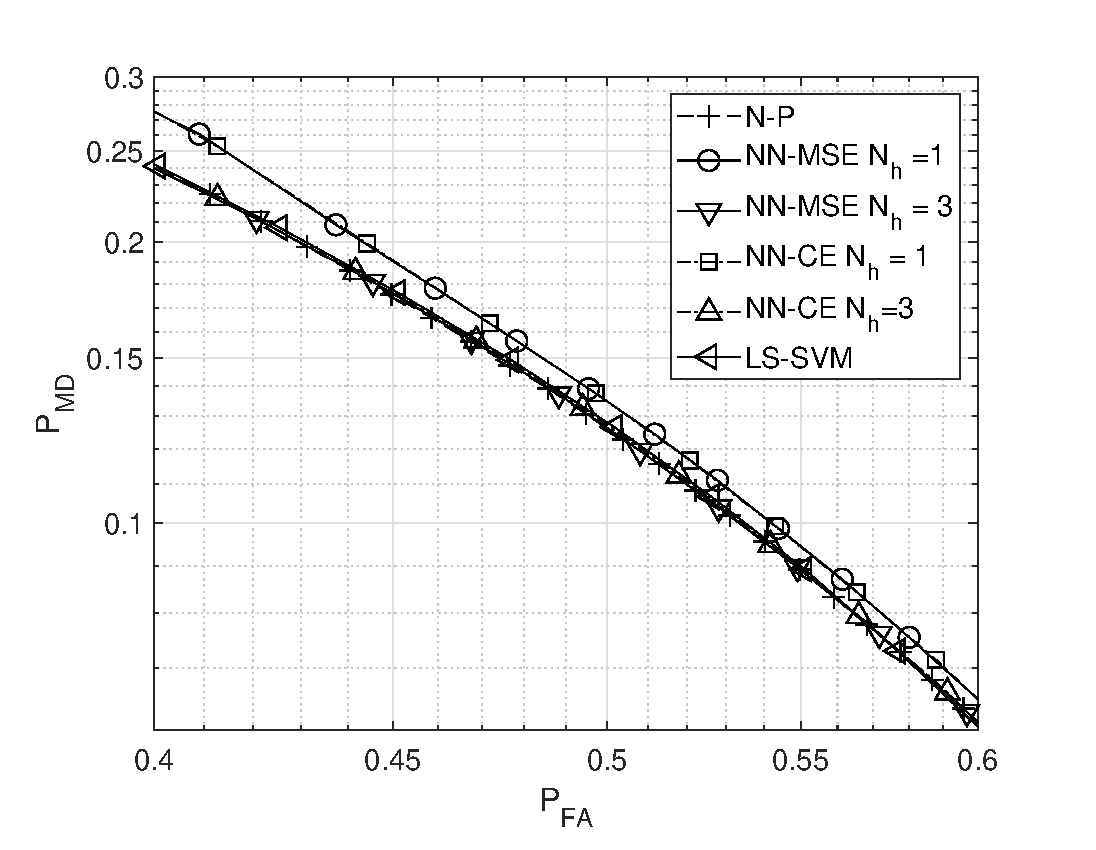
\includegraphics[width=0.5\columnwidth]{res_com_CE_MSE_SVM.eps}
    \caption{$P_{\rm MD}$ vs. $P_{\rm FA}$ obtained in the LOS scenario with a single BS. Comparison between NP detector, \ac{mlp} with \ac{mse} training and CE training and \ac{svm}.}
    \label{fig:ceVSmse}
\end{figure}

Fig. \ref{fig:ceVSmse} shows the \ac{fa} vs. the \ac{md} probabilities obtained by the \ac{irlv} system with $10^6$ training points. In particular we here compare the performance of the \ac{np} detector with the \ac{ml} algorithms. Results for \ac{mlp} are reported for both \ac{mse} and \ac{ce} loss functions. Furthermore we show the performance of the \acp{mlp} with different number of neurons $N_h$ in the hidden layer. We first notice that the \ac{ce}-trained and the \ac{mse}-trained \acp{mlp} obtain the same performance when considering the same number of neurons $N_h$. This confirms that the two training methods are performing hypothesis testing in an equivalent manner. Furthermore we notice that as the number of neurons in the hidden layer grows the performance of the \ac{mlp} classifiers approach those obtained by the \ac{np} classifier, up to the point where they coincide with $N_h=3$ neurons. This shows that both \ac{ce}-trained and \ac{mse}-trained \acp{mlp} at convergence are performing the optimal \ac{np} test and that convergence is obtained with a small number of neurons. Furthermore we notice that the \ac{svm} attains the same performance of the \ac{mlp} with $N_h = 3$ and hence of the \ac{np} detector, confirming that hypothesis testing performed via \ac{svm} is optimal in the \ac{np} sense.




\subsection{No LOS Scenario}\label{sec:res_nLos}
In this section we consider the no-\ac{los} scenario and we show that the \ac{ml}-based solutions are convenient over the \ac{np}-based one.

\begin{figure}[t]
    \centering
    \includegraphics[width=0.5\columnwidth]{surfColorato.png}
    \caption{Example of a realization of the attenuation map in the non-\ac{los} scenario considering only the shadowing effects.}
    \label{fig:map}
\end{figure}

Fig. \ref{fig:map} shows a realization of the attenuation map. A spatial grid has been created in order to take into account the shadowing spatial correlation over different positions. The network includes a single \ac{ap} located at the map center and a squared authentic area $\mathcal{A}_0$, delimited in figure by the red line. Furthermore we consider two \ac{los} paths, one parallel to the $x$ axis and one parallel to the $y$ axis and intersecting at the map center.

Consider the \ac{llr} (\ref{eq:lr}). In the no-\ac{los} context the computation of the two area dependent probabilities has no closed-form solution. A numerical solution is obtained by sampling the attenuation values over the spatial grid of positions and computing the area dependent distributions of the attenuation values. Consider an attenuation value $\hat{a}$: the probability of measuring $\hat{a}$ given that the \ac{ue} is located in area $\mathcal{A}_0$ is given by the number of positions $(x_u,y_u) \in \mathcal{A}_0$ where the measured attenuation $a(x_u,y_u)=\hat{a}$ over the total number of positions $(x_u,y_u)$ in the entire map having the same attenuation $\hat{a}$, i.e.
\begin{equation}
    \mathbb{P}(\hat{a}|\mathcal{A}_0) \approx \frac{\text{number of positions} \, (x_u,y_u) \in \mathcal{A}_0 \, \text{s.t.} \, a(x_u,y_u) = \hat{a}}{\text{total number of positions} \, (x_u,y_u) \, \text{s.t.} \, a(x_u,y_u) = \hat{a}}
\end{equation}
With the same reasoning we compute $\mathbb{P}(\hat{a}|\mathcal{A}_1)$, and an approximation of equation (\ref{eq:lr} is hence obtained as
\begin{equation}\label{eq:lrApp}
    \mathcal{L} \approx \frac{\text{number of positions} \, (x_u,y_u) \in \mathcal{A}_0 \, \text{s.t.} \, a(x_u,y_u) = \hat{a}}{\text{number of positions} \, (x_u,y_u) \in \mathcal{A}_1 \, \text{s.t.} \, a(x_u,y_u) = \hat{a}}
\end{equation}
The value computed by (\ref{eq:lrApp}) gets closer to the real value as the number of grid points over the map increases, as an higher number of points means a better statistical characterization of the attenuation over the map area.

Fig. \ref{fig:trueMap} shows the \ac{md} probability vs. the \ac{fa} probability obtained for the attenuation map in Fig. \ref{fig:map}, where only path loss and shadowing are considered. In particular we here compare the results obtained by (\ref{eq:lrApp}) with the results obtained with \ac{ml}-based approaches. \Ac{mlp} si trained with \ac{mse} loss function and results are shown for different number of neurons $N_h$ in the hidden layer.

In order to compute (\ref{eq:lrApp}) we built a grid with $4.46 \cdot 10^6$ space points, whereas for training the \ac{mlp} and the \ac{svm} we used $10^3$ points. We notice that both the \ac{mlp} and the \ac{svm} achieve better results than the \ac{np}-based detector. This means that the considered number of grid points is not sufficient to approximate the optimal \ac{np} solution. Furthermore we tested the \ac{mlp} with $3$ and $10$ neurons at the hidden layer. We see that with $N_h=10$ the \ac{mlp} and the \ac{svm} attain the same performance. 

\begin{figure}[t]
    \centering
    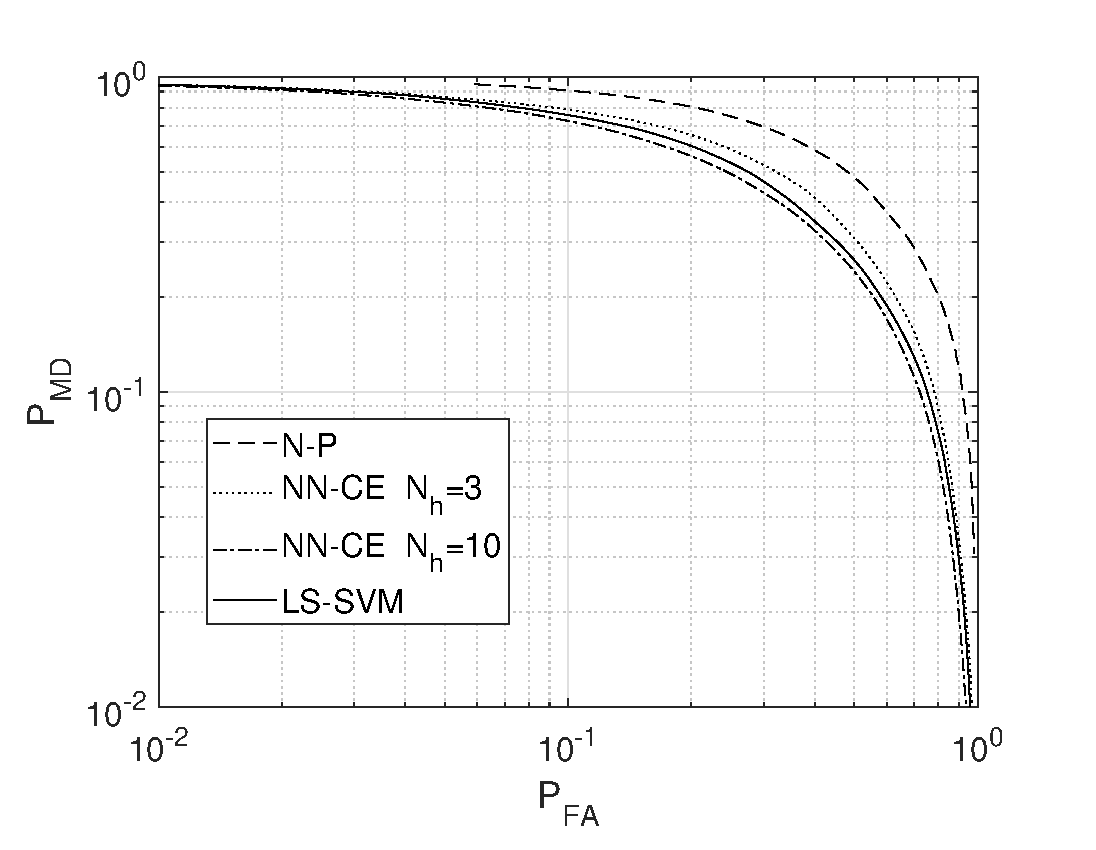
\includegraphics[width=0.5\columnwidth]{res_NP_approx_SVM.eps}
    \caption{$P_{\rm MD}$ vs. $P_{\rm FA}$ for the attenuation map in Fig. \ref{fig:map}. Comparison between the \ac{np}-based and the \ac{ml}-based detectors}
    \label{fig:trueMap}
\end{figure}

Comparing the number of grid points and the number of training points used for the \ac{ml} algorithms we can conclude that the \ac{ml}-based solution is advantageous over the \ac{np}-based one, as it requires a smaller number of points in order to get an estimate of the area dependent probabilities. Furthermore this implies that the \ac{ml}-based \ac{irlv} system can be implemented without any a-priory knowledge of the \ac{pdf} of the hypothesis to be tested.

\subsection{Fading Effects}\label{sec:res_fading}

Consider the network in Fig. \ref{fig:mBS}. $N_{\rm ap}=5$ \acp{ap} gather attenuation values from the \acp{ue}. Each \ac{ap} gathers the attenuation value of the transmitting \ac{ue} and sends it to the central unit, which builds the attenuation vector $\bm{a}$ that is used for \ac{irlv}. In order to compute the \ac{llr} in (\ref{eq:lr}) we should here consider a $N_{\rm AP}$-dimensional multivariate Gaussian distribution. However, as the \ac{llr} equation in this case has no closed-form solution and since we showed in \ref{sec:res_nLos} that the \ac{ml}-based solutions achieve the optimal results of the \ac{np} detector with a smaller number of training points, we only show here results for the \ac{ml}-based solutions.

\begin{figure}[t]
    \centering
    \includegraphics[width=0.3\columnwidth]{scenario2.png}
    \caption{Scenario with multiple BSs: each one gathers the attenuation value of the transmitting user and passes it to the central unit that builds the attenuation vector $\bm{a}$ used for discriminating the location of the user.}
    \label{fig:mBS}
\end{figure}
\begin{figure}[t]
    \centering
    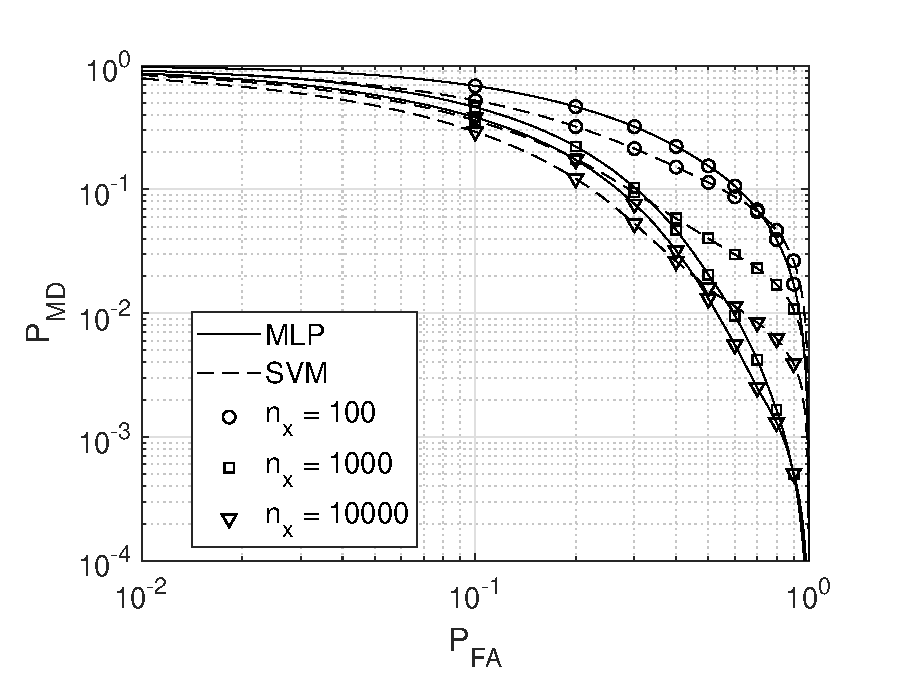
\includegraphics[width=0.5\columnwidth]{res_avg_nTrain_kf1.eps}
    \caption{$P_{\rm MD}$ vs. $P_{\rm FA}$ for different training set size and $k_f=1$ fading realization. The \ac{mlp} is implemented with $N_h = 10$ and \ac{ce} loss function}
    \label{fig:kf1}
\end{figure}

\begin{figure}[t]
    \centering
    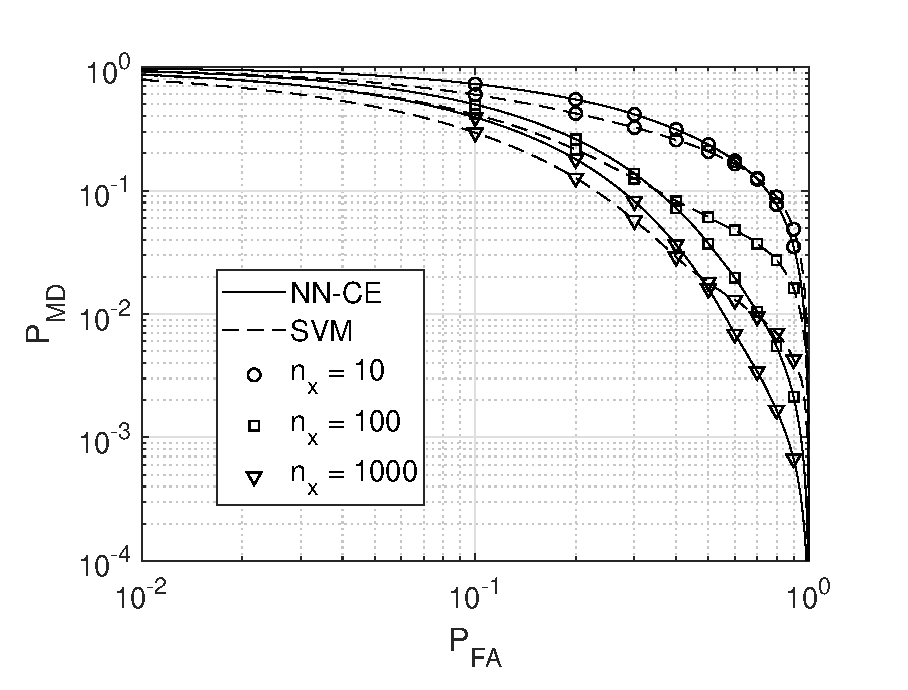
\includegraphics[width=0.5\columnwidth]{res_avg_nTrain_kf10.eps}
    \caption{$P_{\rm MD}$ vs. $P_{\rm FA}$ for different training set size and $k_f=10$ fading realizations. The \ac{mlp} is implemented with $N_h = 10$ and \ac{ce} loss function}
    \label{fig:kf10}
\end{figure}

In order to build the training set we consider $n_x$ spatial points $\bm{x}_{\rm ue}$, each one representing the coordinates of the position of a \ac{ue}, uniformly distributed over the attenuation map. Consider a realization of the shadowing map as depicted in Fig. \ref{fig:map}. A single position $\bm{x}_{\rm ue}$ is associated to a single shadowing value, however since we also include fading effects, the attenuation vectors measured by the \acp{ap} in different time instants for $\bm{x}_{\rm ue}$ assume different value, do to the independent fading realizations. We define the size of the training set as the value $k_t = n_x \cdot k_f$, which considers $n_x$ spatial coordinates and $k_f$ fading realizations for each $\bm{x}_{\rm ue}$.

We consider and compare two realizations of the training set: the former considering a single fading realization for each spatial coordinate; the latter considering $k_f > 1$ fading realization for each spatial coordinate. 

Fig.s \ref{fig:kf1} and \ref{fig:kf10} show the effect of $k_f$ on the \ac{irlv} system performance. In particular, they show the $P_{\rm MD}$ vs. $P_{\rm FA}$ for different numbers of considered spatial coordinates and fixed $k_f$. Results are reported in solid line for the \ac{mlp} and in dashed line for the \ac{svm} . The \ac{mlp} has been implemented with $N_h=10$ and \ac{ce} loss function. Different markers denote different training set size values $k_t$. Comparing the performance in the two figures we notice that, for a given training set value $k_t$, performance get worse as the number of fading realization increase. However we also notice that, for a given number of spatial position $n_x$, performance are better if we consider a larger number of fading realizations. Furthermore we see that, for a large enough training set, performance for different values $k_f$ are approximately the same. This implies that, if the training set is large enough, the \ac{ml} algorithms are also robust to noise, as they are able to average out the fading component affecting a single position and ensuring the same performance for the two differently built training sets. 


\section{Numerical Results: One Class Classification}
We here present numerical results for the scenario where the available data for training comes only from one of the two regions. 

Considering the \ac{ae}, the performance of the \ac{irlv} system depend on the compressing capability of the \ac{ae} and hence on the number of neurons $N_h$ in the hidden layer. Consider the scenario depicted in Fig. \ref{fig:mBS}, where the \ac{irlv} system procedure is the same described in previous sections. Fig. \ref{fig:aeNh} shows the $P_{\rm FA}$ vs. the $P_{\rm MD}$ probabilities for the \ac{ae} for different number of neurons $N_h$. The \ac{ae} has been trained with $k_t=10^4$ training vectors. Fading effects are not considered in this case. We see that for the \ac{ae} increasing the number of neurons $N_h$ do not lead to better \ac{irlv} system performance as seen for the \ac{mlp}. In fact we notice that the best performance are obtained for $N_h=2$ and that the performance get worse are $N_h$ further increases. This is due to the fact that the \ac{ae} is performing compression of the attenuation vectors and hence needs to extract an optimal number of features from the input values. From Fig. \ref{fig:aeNh} we can conclude that the optimal number of features to be extracted is $2$, whereas considering a larger number of features is over-representative of the input model and hence lead to worse system performance.

\begin{figure}[t]
    \centering
    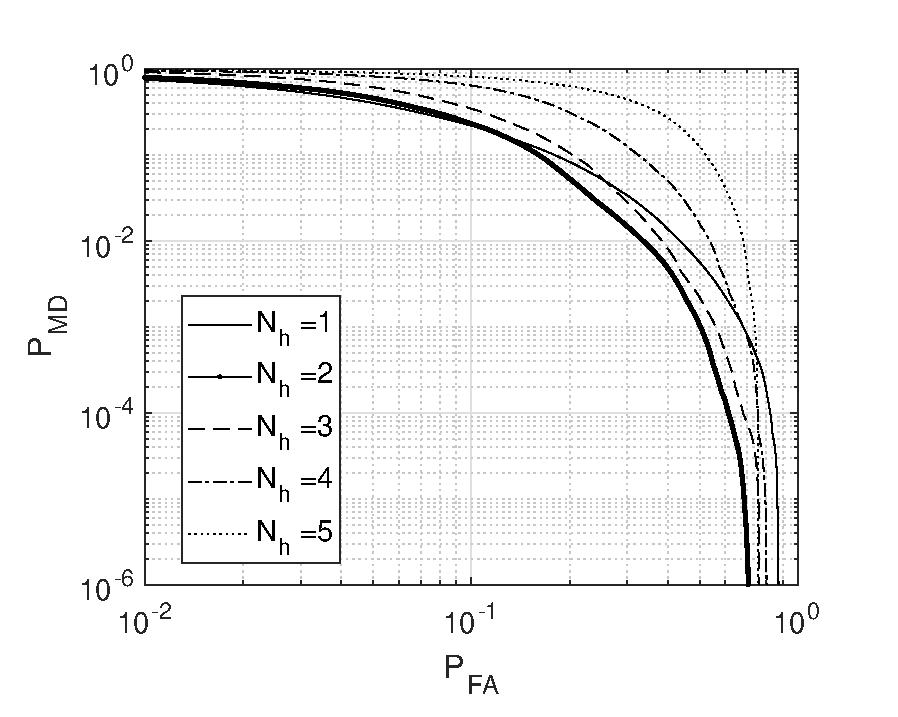
\includegraphics[width=0.5\columnwidth]{res_ae_onNeur.eps}
    \caption{$P_{\rm MD}$ vs. $P_{\rm FA}$ for the \ac{ae} with different values of $N_h$, $k_t=10^4$ and no fading.}
    \label{fig:aeNh}
\end{figure}

\subsection{Fading Effects}
We here consider the effect of the training set size $k_t$ on the system performance for the one class classification based \ac{irlv}. Consider the scenario depicted in Fig. \ref{fig:mBS} where the \ac{irlv} system gathers attenuation vectors as described in the previous sections. For the one class classification the training set is built only with attenuation vectors collected from user located in area $\mathcal{A}_0$, whereas the testing set is composed by both attenuation vectors measured from area $\mathcal{A}_0$ and area $\mathcal{A}_1$. As for \ref{sec:res_fading} we consider a training set with size $k_t = n_x \cdot k_f$ and we test and compare the training sets created with $k_f=1$ and $k_f >1$.

Fig.s \ref{fig:kf1Oc} and \ref{fig:kf10Oc} show the performance of the \ac{irlv} system for both \ac{ae} and \ac{oclssvm} respectively for $k_f = 1$ and $k_f = 10$. In particular, they show the $P_{\rm MD}$ vs. $P_{\rm FA}$ for different numbers of considered spatial coordinates and fixed $k_f$. Results are reported in solid line for the \ac{ae} and in dashed line for the \ac{oclssvm} . The \ac{ae} has been implemented with $N_h=2$. Different markers denote different training set size values $k_t$.

We first notice that the \ac{ae} is less sensitive to the training set size, as different values of $k_t$ attains the same performance for $k_f=1$ and approximately the same performance for $k_f = 10$. Furthermore we notice that, for values $P_{\rm FA} > 10^{-1}$ the \ac{oclssvm} attains lower values of $P_{\rm MD}$. Comparing the performance obtained by the two algorithms for fixed $k_t$ and different $k_f$ values we notice that the \ac{ae} is not sensitive to noise, as the error probabilities are almost the same in the two figures. Instead we notice that the \ac{oclssvm} is more sensitive to noise when the training set size is small. In fact we notice that for $k_t=10^2$ performance are different for $k_f=1$ and $k_f=10$. Instead, when $k_t$ grows, performance are almost the same for both values of $k_f$. Furthermore we notice that, when the training set size is small it is convenient to build the training set for the \ac{oclssvm} considering a single time instant for each $\bm{x}_{\rm ue}$, i.e, with $k_f = 1$. Differently from what obtained for the two class case, we see that with \ac{oclssvm}, by fixing the value $n_x$ the performance obtained for different values of $k_f$ are almost the same, meaning that it is not convenient in terms of error probabilities to measure different fading realizations for all the spatial positions.

Comparing the results obtained for the one class classification with those obtained by the two class classification (Fig.s \ref{fig:kf1} and \ref{fig:kf10}) we notice that the performance obtained by the \ac{svm}-based algorithms the one class classification performs better than two class when considering large training sets for both values of $k_f = 10$ and $P_{\rm FA}>10^{-1}$. When considering the \ac{nn}-based algorithms we see that one class classification performs better than the two-class for small training set size and viceversa for larger $k_t$ values and $P_{\rm FA} > 10^{-1}$. This result holds for both values of $k_f$. Furthermore we see that the \ac{oclssvm} attains better performance than those obtained by the \ac{mlp} when considering the same values of $n_x$ and $k_f$ and $P_{\rm FA}> 10^{-1}$.


\begin{figure}[t]
    \centering
    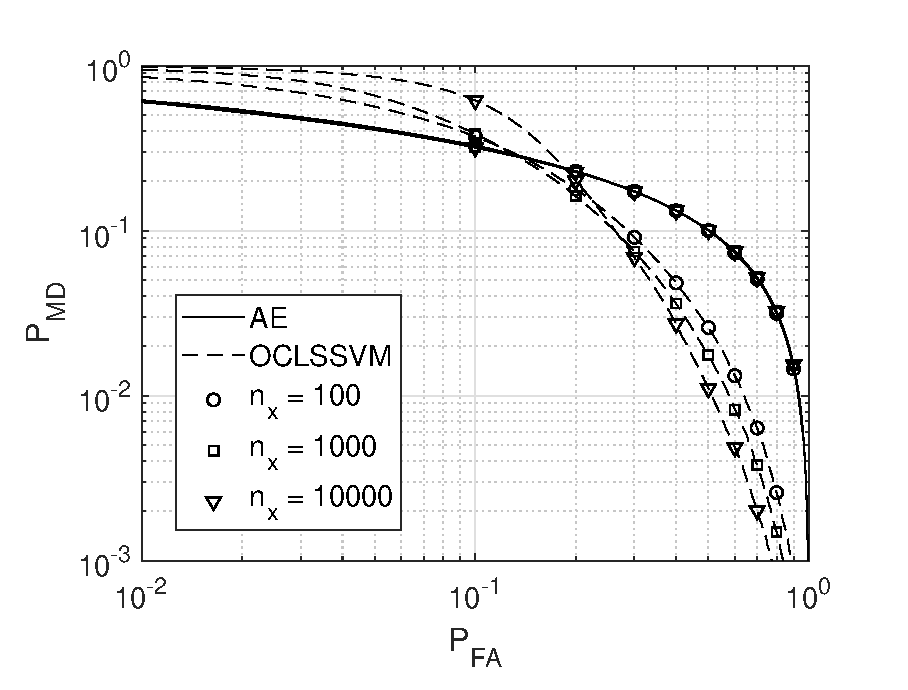
\includegraphics[width=0.5\columnwidth]{res_avgnTrain_oneClass_kf1.eps}
    \caption{Convergence of the \ac{ae}. $P_{\rm MD}$ vs. $P_{\rm FA}$ for \ac{ae} with $N_h = 2$, different training set size and $k_f=10$ fading realizations.}
    \label{fig:kf1Oc}
\end{figure}

\begin{figure}[t]
    \centering
    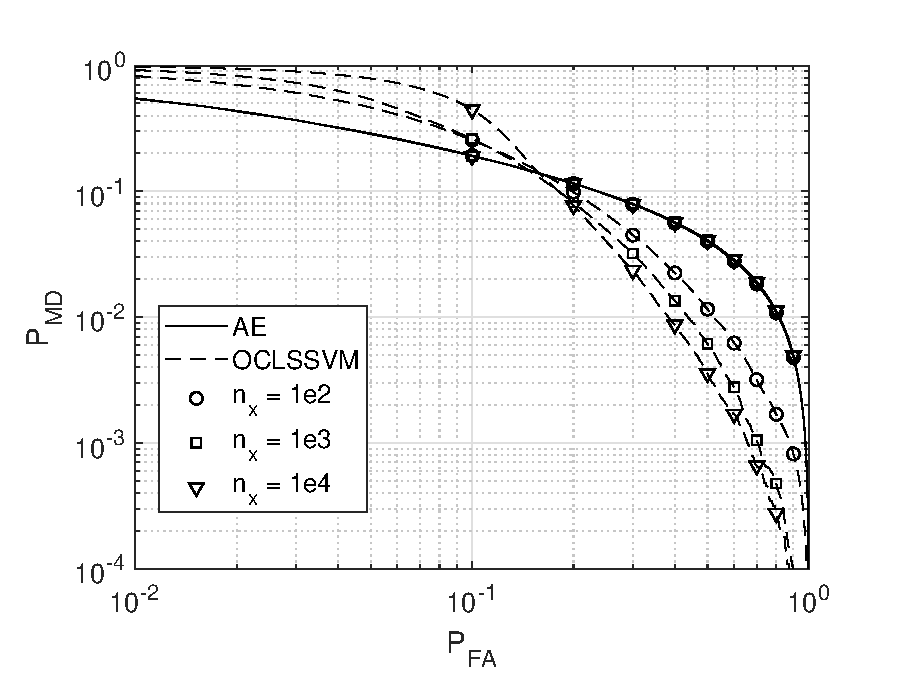
\includegraphics[width=0.5\columnwidth]{res_avgnTrain_oneClass_kf10.eps}
    \caption{Convergence of the \ac{ae}. $P_{\rm MD}$ vs. $P_{\rm FA}$ for \ac{ae} with $N_h = 2$, different training set size and $k_f=10$ fading realizations.}
    \label{fig:kf10Oc}
\end{figure}

\section{Numerical Results: Attack Strategies}
Consider the scenario depicted in Fig. \ref{fig:mBS}, where $N_{\rm AP}=5$ \acp{ap} gather attenuation vectors from the transmitting users. Consider attenuation vectors composed by path loss and shadowing, where fading effects are not taken into account. Both attack and defense are trained with one class classifier, respectively trained with attenuation vectors measured from $\mathcal{A}_1$ and $\mathcal{A}_0$. In order to test the attacks we fix a \ac{fa} probability at the defense side, such that the threshold value needed for classification is given. We compare attacks and defense both implemented via \ac{ae} and \ac{oclssvm}. 

In order to test the proposed attack strategies we compare them with random attacks, i.e., where attenuation vectors appointed for attack are selected by randomly choosing a position in the non legitimate area $\mathcal{A}_1$. In particular we consider two different random attacks: the former generates random positions in the overall area $\mathcal{A}_1$, the latter generates random positions in the portion of area $\mathcal{A}_1$ which is at the border of the legitimate area $\mathcal{A}_0$. 

\section*{Appendix}

	Given a finite alphabet $\mathcal A = \{\bm{\alpha}_1, \ldots, \bm{\alpha}_M\}$ of $M$ elements for $\bm{a}^{(i)}$, we indicate with $p_{\bm{a}^{(i)},t_i}(\bm{\alpha}_j, t)$, with $t \in \{-1,1\}$, the joint probability of input vector $\bm{a}^{(i)}$ and corresponding output $t_i$, $i=1, \ldots, S$.
	
	By the Glivenko–Cantelli theorem we have that with probability 1 as $S\rightarrow \infty$ there are $Sp_{\bm{a}^{(i)},t_i}(\bm{\alpha}_j,t)$ training vectors $\bm{\alpha}_j$ with associated true value $t$ in any training sequence.
	All these training points will have the same value $e_i$, from (\ref{eq:stpart}), that will appear $Sp_{\bm{a}^{(i)},y_i}(\bm{\alpha}_j,t)$ times in the sum $\sum_{i=1}^{S} e_i^2$.
	Note that in the training ensemble there could be two equal instances $\bm{a}^{(m)}=\bm{a}^{(n)}=\bm{\alpha}_j$, but with different labels $t_m \neq t_n$. Therefore, for $\bm{a}^{i}=\bm{\alpha}_j$ we can have two possible values for $e_i$, depending on $y_i$, and we denote them with $e_{j,1}$ and $e_{j,-1}$.
	This translates in only $2M$ \textit{distinct} constraints of the type \eqref{eq:stpart}.
	Asymptotically, for $S \to \infty$, problem (\ref{eq:lssvm}) becomes
	\begin{subequations}
		\label{eq:lssvm22}
		\begin{equation}
		\label{eq:lssvm2}
		\underset{\bm{w},e}{\text{min}} \quad f_l' \triangleq \frac{1}{2} \bm{w}^T \bm{w} + C S \frac{1}{2} \sum_{j=1}^M [p_{\bm{a}^{(i)},t_i}(\bm{\alpha}_j,1) e_{j,1}^2 + p_{\bm{a}^{(i)},y_i}(\bm{\alpha}_j,-1) e_{j,-1}^2]  
		\end{equation}
		subject to 
		\begin{equation}
		\label{eq:stpart2}
		[\bm{w}^T \phi (\bm{\alpha}_j) + b] = 1- e_{j,1}\quad j = 1 ,\dots,M.
		\end{equation}
		\begin{equation}
		\label{eq:stpart3}
		\quad  -[\bm{w}^T \phi (\bm{\alpha}_j) + b] = 1- e_{j,-1}\quad j = 1 ,\dots,M.
		\end{equation}
	\end{subequations}
	whose solution provides the convergence value (in probability) of vector $\bm{w}$. We write the Lagrangian
	\begin{equation}
	\mathcal{L}_1 = f_l' - \sum_{k=1}^{M} v_k \left[ \bm{w}^T \phi (\bm{\alpha}_j) + b - 1 + e_{j,1} \right] 
	- \sum_{k=1}^{M} u_k \left[- \bm{w}^T  \phi (\bm{\alpha}_j) - b  - 1 + e_{j,-1} \right], 
	\end{equation}
	where $\{u_k,v_k\}_{k=1}^{M}$ are the Lagrangian multipliers. Let us set to zero the derivatives w.r.t. $\{\bm{w},b,e_{j,1},e_{j,-1}, v_j,u_j\}$
	\begin{subequations}
		\begin{equation}
		\label{eq:deriv1_1}
		\frac{\partial \mathcal{L}_1}{ \partial \bm{w}}: \quad \bm{w} = \sum_{k=1}^{M} (u_k - v_k) \phi (\bm{\alpha}_k),
		\end{equation}
		\begin{equation}
		\label{eq:deriv1_2}
		\frac{\partial \mathcal{L}_1}{\partial b}: \quad \sum_{k=1}^{M} (u_k - v_k) = 0 ,
		\end{equation}
		\begin{equation}
		\label{eq:deriv1_3}
		\frac{\partial \mathcal{L}_1}{\partial e_{j,1}}: \quad v_j = CSp_{\bm{a}^{(i)},t_i}(\bm{\alpha}_j,1) e_{j,1} \quad j=1\dots M,
		\end{equation}
		\begin{equation}
		\label{eq:deriv1_4}
		\frac{\partial \mathcal{L}_1}{\partial e_{j,-1}}: \quad u_j = CSp_{\bm{a}^{(i)},t_i}(\bm{\alpha}_j,-1) e_{j,-1} \quad j=1\dots M,
		\end{equation}
		\begin{equation}
		\label{eq:deriv1_5}
		\frac{\partial \mathcal{L}_1}{\partial v_j}: \quad \bm{w}^T \phi (\bm{\alpha}_j) + b - 1 + e_{j,1} = 0 \quad j=1\dots M,
		\end{equation}
		\begin{equation}
		\label{eq:deriv1_6}
		\frac{\partial \mathcal{L}_1}{\partial u_j}: \quad - \bm{w}^T \phi (\bm{\alpha}_j) - b - 1 + e_{j,-1} = 0 \quad j=1\dots M.
		\end{equation}
	\end{subequations}
	Substituting \eqref{eq:deriv1_1}, \eqref{eq:deriv1_3} and \eqref{eq:deriv1_4} in \eqref{eq:deriv1_5} and \eqref{eq:deriv1_6} we get the system of equations
	\begin{subequations}
		\label{eq:system1}
		\begin{equation}
		\sum_{k=1}^{M} (u_k - v_k) k(\phi (\bm{\alpha}_k,\bm{\alpha}_j)) + b - 1 + \frac{v_j}{CSp_{\bm{a}^{(i)},t_i}(\bm{\alpha}_j,1)} = 0
		\quad j=1\dots M
		\end{equation}
		\begin{equation}
		- \sum_{k=1}^{M} (u_k - v_k) k(\phi (\bm{\alpha}_k,\bm{\alpha}_j)) - b - 1 + \frac{v_j}{CSp_{\bm{a}^{(i)},t_i}(\bm{\alpha}_j,-1)} = 0
		\quad j=1,\dots, M
		\end{equation}
		\begin{equation}
		\sum_{k=1}^{M} (u_k - v_k) = 0.
		\end{equation}
	\end{subequations}
	\eqref{eq:system1} is a system with $2M + 1$ equations, linear in the $2M + 1$ unknowns $\{u_k,v_k,b\}_{k=1}^{k=M}$ and therefore has finite solution. In particular, using \eqref{eq:deriv1_1}, we have
	\begin{equation}
	\label{eq:wSolution}
	\bm{w}^T\bm{w} =  \sum_{k=1}^{M} \sum_{h=1}^{M} k(\bm{\alpha}_k,\bm{\alpha}_h) (v_kv_h + u_ku_h -2 v_ku_h),
	\end{equation}
	where we used the fact that the kernel function
	\begin{equation}
	k(\bm{\alpha}_k,\bm{\alpha}_h) \triangleq \phi(\bm{\alpha}_k) \phi(\bm{\alpha}_h)^T
	\end{equation}
	 is symmetric \wrt its inputs. 
	
%	Note that while the original problem \eqref{eq:lssvm}, as $S \to \infty$, has infinite constraints, the equivalent formulation \eqref{eq:lssvm22} includes a finite number $2M$ of constraints.
	
	We conclude that $\bm{w}$ has a finite norm since the rhs of \eqref{eq:wSolution} is a finite sum.
	 
\newpage 



%\bibliographystyle{IEEEtran}
%\bibliography{bibliography.bib}
\renewcommand*{\bibfont}{\footnotesize}

\printbibliography

\end{document}
